% Filename: cap01@notas_de_aula.tex
% This code is part of 'Notas de aula n\~{a}o oficiais de MS650 e F620'
% 
% Description: This file correspond to part of the textbook using in the course.
% 
% Created: 02.08.12 10:36:23 PM
% Last Change: 02.08.12 10:36:23 PM
% 
% Authors:
% - Raniere Silva, r.gaia.cs@gmail.com
% 
% Copyright (c) 2012, Raniere Silva. All rights reserved.
% 
% This work is licensed under the Creative Commons Attribution-NonCommercial-NoDerivs 3.0 Unported License. To view a copy of this license, visit http://creativecommons.org/licenses/by-nc-nd/3.0/.
%
% This work is distributed in the hope that it will be useful, but WITHOUT ANY WARRANTY; without even the implied warranty of MERCHANTABILITY or FITNESS FOR A PARTICULAR PURPOSE.
%
\chapter{S\'{e}ries de Fourier}
A s\'{e}rie
\begin{align*}
    \frac{A_0}{2} + \sum_{n = 1}^\infty \left( A_n \cos\left( n x \right) + B_n \sin\left( n x \right) \right)
\end{align*}
\'{e} chamada uma s\'{e}rie trigonom\'{e}trica.

\begin{defi}
    A s\'{e}rie trigonom\'{e}trica
    \begin{align*}
        \frac{a_0}{2} + \sum_{n = 1}^\infty \left( a_n \cos\left( n x \right) + b_n \sin\left( n x \right) \right)
    \end{align*}
    \'{e} a s\'{e}rie de Fourier da fun\c{c}\~{a}o $f(x)$ se os coeficientes forem dados por
    \begin{align*}
        a_n &= \frac{1}{n} \int_{-\pi}^\pi f(x) \cos\left( n x \right) \id{x} && n = 0, 1, 2, \ldots \\
        b_n &= \frac{1}{\pi} \int_{-\pi}^\pi f(x) \sin\left( n x \right) \id{x} && n = 1, 2, \ldots
    \end{align*}
\end{defi}

Algumas quest\~{o}es:
\begin{enumerate}
    \item a s\'{e}rie converge?
    \item qual o intervalo de converg\^{e}ncia?
    \item qual o tipo de converg\^{e}ncia?
        \begin{exem}
            Para a converg\^{e}ncia uniforme temos que $\forall \epsilon > 0, \exists n > 0$ tal que $| \delta_m(x) - \delta_n(x)| < \epsilon$ sempre que $m, n > N, \forall x \in I$ (onde $\delta_n(x) = \sum_{k = 1}^\nu \mu_k(x)$).
        \end{exem}
    \item quais fun\c{c}\~{o}es $f(x)$ s\~{a}o respresent\'{a}veis por essa s\'{e}rie? Condi\c{c}\~{o}es sobre $f(x)$?
\end{enumerate}

Um fato not\'{a}vel \'{e} que as condi\c{c}\~{o}es para representar uma fun\c{c}\~{a}o por uma s\'{e}rie de Fourier s\~{a}o menos restritivas do que para s\'{e}ries de pot\^{e}ncias.

\begin{obs}
    Temos que $\left\{ \cos\left( n x \right), \sin\left( n x \right) \right\}$ s\~{a}o fun\c{c}\~{o}es peri\'{o}dicas com $T = 2\pi$ e portanto $f(x)$ \'{e} uma fun\c{c}\~{a}o peri\'{o}dica, i.e., $f(x + 2\pi) = f(x)$.
\end{obs}

\begin{exem} \label{exem:fourier:x^2}
    Para $f(x) = x^2$ temos que
    \begin{align*}
        a_0 &= \frac{1}{\pi} \int_{-\pi}^\pi x^2 \id{x} = \frac{1}{\pi} \left. \frac{x^3}{3} \right|_{-\pi}^\pi = \frac{2 \pi^2}{3}, \\
        a_n &= \frac{1}{n} \int_{\pi}^\pi x^2 \cos\left( n x \right) \id{x} \\
        &= \frac{1}{\pi} \left[ \underbrace{\left. \frac{x^2 \sin\left( n x \right)}{n} \right|_{-\pi}^\pi}_{= 0} - \frac{1}{n} \int_{-\pi}^\pi 2 x \sin\left( n x \right) \id{x} \right] \\
        &= \frac{-1}{n \pi} \left[ \left. \frac{-2 x \cos\left( n x \right)}{n} \right|_{-\pi}^\pi + \frac{1}{n} \int_{-\pi}^\pi 2 \cos\left( n x \right) \id{x} \right] \\
        &= \frac{-1}{n \pi} \left[ \frac{-2 \pi \cos\left( n \pi) \right)}{n} + \frac{2 (-\pi) \cos(n) (-\pi)}{n} + \frac{2}{n} \underbrace{\left. \frac{\sin\left( n x \right)}{n} \right|_{-\pi}^\pi}_{= 0} \right] \\
        &= \frac{-1}{n \pi} \left[ \frac{- 4 \pi}{n} \cos\left( n \pi \right) \right] \\
        &= \frac{4}{n^2} (-1)^n, \\
        b_n &= \frac{1}{n} \int_{-\pi}^\pi x^2 \sin\left( n x \right) \id{x} \\
        &= \frac{1}{\pi} \left[ \left. \frac{- x^2 \cos\left( n x \right)}{n} \right|_{-\pi}^\pi + \frac{1}{n} \int_{-\pi}^\pi 2 x \cos\left( n x \right) \id{x} \right] \\
        &= \frac{1}{n} \left[ \frac{-\pi^2 \cos\left( n \pi \right)}{n} + \frac{\pi \cos\left( n (-\pi) \right)}{n} + \frac{1}{n} \int_{-\pi}^\pi 2 x \cos\left( n x \right) \id{x} \right] \\ 
        &= \frac{1}{n} \left[ \frac{1}{n} \left[ \underbrace{\left. \frac{2 x \sin\left( n x \right)}{n} \right|_{-\pi}^\pi}_{= 0} - \frac{1}{n} \underbrace{\int_{-\pi}^\pi 2 \sin\left( n x \right) \id{x}}_{= 0} \right] \right] \\
        &= 0,
    \end{align*}
    onde $n > 0$.

    Logo,
    \begin{align*}
        x^2 = \frac{\pi^2}{3} + \sum_{n = 1}^\infty \frac{4 (-1)^n}{n^2} \cos\left( n x \right).
    \end{align*}
\end{exem}

\begin{obs}
    Essa s\'{e}rie representa $f(x) = x^2$ para $-\pi \leq x \leq \pi$. Para os demais pontos trata-se da extens\~{a}o peri\'{o}dica de $f(x) = x^2$, $-\pi \leq x \leq \pi$.
\end{obs}

\begin{figure}[!htb]
    \centering
    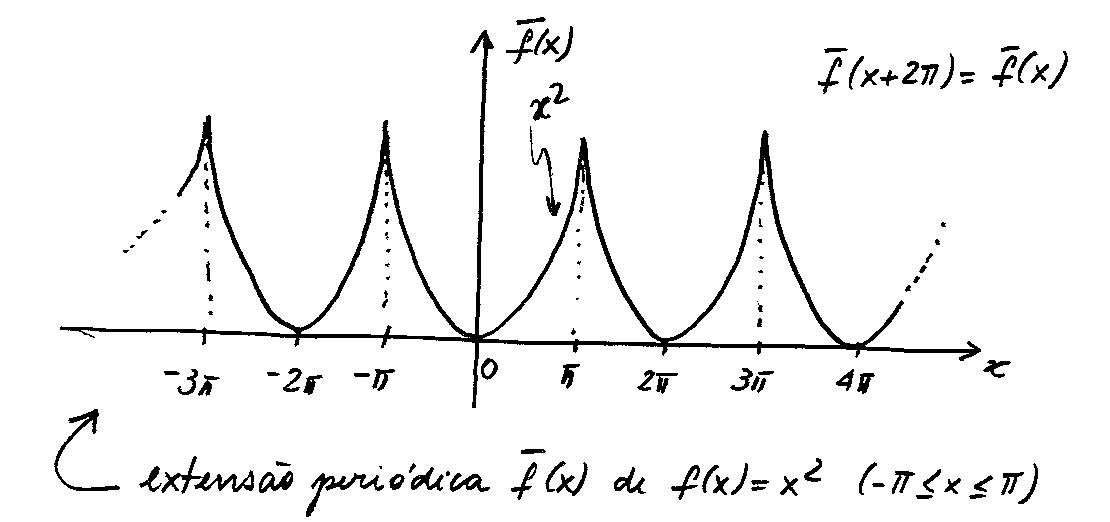
\includegraphics[width=0.8\textwidth]{figuras/serie_fourier_grafico01.jpg}
    \caption{Gr\'{a}fico da s\'{e}rie de Fourier para $f(x) = x^2$.}
    \label{fig:serie_fourier_grafico01}
\end{figure}

\begin{exem}
    Para
    \begin{align*}
        f(x) &= \begin{cases}
            -1, & x < 0, \\
            +1, & x \geq 0.
        \end{cases}
    \end{align*}
    temos que
    \begin{align*}
        a_0 &= \frac{1}{\pi} \int_{-\pi}^\pi f(x) \id{x} \\
        &= \frac{1}{\pi} \left[ -\int_\pi^0 \id{x} + \int_0^\pi \id{x} \right] \\
        &= 0, \\
        a_n &= \frac{1}{\pi} \int_{-\pi}^\pi f(x) \cos\left( n x \right) \id{x} \\
        &= \frac{1}{n} \left[ -\int_{-\pi}^0 \cos\left( n x \right) \id{x} + \int_0^\pi \cos\left( n x \right) \id{x} \right] \\
        &= 0, \\
        b_n &= \frac{1}{\pi} \int_{-\pi}^\pi f(x) \sin\left( n x \right) \id{x} \\
        &= \frac{1}{\pi} \left[ -\int_{-\pi}^0 \sin\left( n x \right) \id{x} + \int_0^\pi \sin\left( n x \right) \id{x} \right] \\
        &= \frac{2}{\pi} \int_0^\pi \sin\left( n x \right) \id{x} \\
        &= \left. \frac{-2 \cos\left( n x \right)}{n \pi} \right|_0^\pi \\
        &= \frac{-2}{n \pi} \left[ (-1)^n - 1 \right] \\
        &= \begin{cases}
            0, & n \text{ \'{e} par}, \\
            4 / \left( n \pi \right), & n \text{ \'{e} \'{i}mpar}.
        \end{cases}
    \end{align*}

    Logo,
    \begin{align*}
        f(x) &= \sum_{n = 1}^\infty b_n \sin\left( n x \right) \\
        &= \sum_{k = 1}^\infty b_{k + 1} \sin\left( (2k + 1) x \right) \\
        &= \sum_{k = 0}^\infty \frac{4}{\left( 2k + 1 \right) \pi} \sin\left( (2k + 1) x \right).
    \end{align*}
\end{exem}

\begin{figure}[!htb]
    \centering
    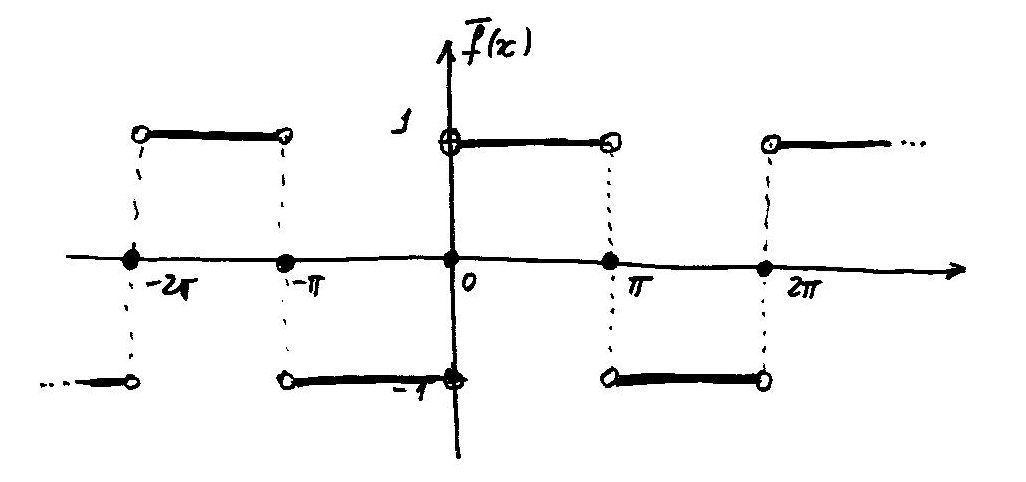
\includegraphics[width=0.8\textwidth]{figuras/serie_fourier_grafico02.jpg}
    % TODO Arrumar o comando \caption abaixo.
    \caption{Gr\'{a}fico da s\'{e}rie de Fourier para }
    \label{fig:serie_fourier_grafico02}
\end{figure}

Pela Figura~\ref{fig:serie_fourier_grafico02} que
\begin{align*}
    \bar{f}(x) &= \begin{cases}
        1, & 0 < x < \pi, \\
        0, & x = 0, \pi, -\pi, \\
        -1, & -\pi < x < 0.
    \end{cases}
\end{align*}
e
\begin{align*}
    \bar{f}(x + 2 \pi) &= \bar{f}(x).
\end{align*}

\begin{obs}
    $\bar{f}(0) \neq f(0)$, o que \'{e} caractyeristico do comportamento da s\'{e}rie de Fourier em uma descontinuidade. Note que
    \begin{align*}
        \bar{f}(0) &= \frac{1}{2} \left[ \lim_{x \to 0^+} f(x) + \lim_{x \to 0^-} f(x) \right]
    \end{align*}
    nesse caso (que se mostrar\'{a} verdade no caso geral!).
\end{obs}

\begin{defi}
    Seja $\mathcal{L}^2[a, b]$ o conjunto das fun\c{c}\~{o}es de quadrado integr\'{a}vel em $a \leq x \leq b$. Dizemos que $f(x)$ e $g(x)$ s\~{a}o ortogonais nesse intervalo se
    \begin{align*}
        \int_a^b f(x) g(x) \id{x} &= 0.
    \end{align*}
\end{defi}

\begin{obs}
    Lembrando que
    \begin{align*}
        0 \leq \left( f - g \right)^2 = f^2 + g^2 - 2 f g,
    \end{align*}
    ou seja,
    \begin{align*}
        2 f g \leq f^2 + g^2,
    \end{align*}
    conclu\'{i}mos que se $f, g \in \mathcal{L}^2[a, b]$, ent\~{a}o existe $\int_a^b f(x) g(x) \id{x}$. Al\'{e}m disso,
    \begin{align*}
        \left( f + g \right)^2 &= f^2 + g^2 + 2 f g \leq 2 \left( f^2 + g^2 \right),
    \end{align*}
    o que garante que $f + g \in \mathcal{L}^2[a, b]$. Como $\mathcal{L}^2[a, b]$ \'{e} um espa\c{c}o vetorial, podemos pesnar nessa integral como o produto escalar $<f, g>$ de $f, g \in \mathcal{L}^2[a, b]$:
    \begin{align*}
        <f, g> = \int_a^b f(x) g(x) \id{x}.
    \end{align*}
\end{obs}

\begin{prop}
    O conjunto $\left\{ 1, \cos\left( n x \right), \sin\left( n x \right) \right\}$ ($n = 1, 2, \ldots$) \'{e} ortogonal em $[-\pi, \pi]$.
\end{prop}
\begin{proof}
    Devemos mostrar que
    \begin{align}
        & \int_{-\pi}^\pi 1 \cos\left( n x \right) \id{x} = \int_{-\pi}^\pi 1 \sin \left( n x \right) \id{x} = 0, \tag{i} \label{eq:serie_fourier_ort01} \\
        & \int_{-\pi}^\pi \cos\left( n x \right) \cos\left( m x \right) \id{x} = \int_{-\pi}^\pi \sin\left( n x \right) \sin\left( m x \right) \id{x} = 0, n \neq m, \tag{ii} \label{eq:serie_fourier_ort02} \\
        & \int_{-\pi}^\pi \cos\left( n x \right) \sin\left( m x \right) \id{x} = 0. \tag{iii} \label{eq:serie_fourier_ort03}
    \end{align}
    As integrais \eqref{eq:serie_fourier_ort01} s\~{a}o triviais. Quanto a \eqref{eq:serie_fourier_ort02} e \eqref{eq:serie_fourier_ort03}, elas s\~{a}o calculadas de forma an\'{a}loga, de modo que faremos explicitamente apenas uma delas. Usando a identidade
    \begin{align*}
        \cos\left( n x \right) \cos\left( m x \right) &= \frac{1}{2} \cos\left( (n - m) x \right) + \frac{1}{2} \cos\left( (n + m) x \right)
    \end{align*}
    segue, para $n \neq m$, que
    \begin{align*}
        \int_{-\pi}^\pi \cos\left( n x \right) \cos\left( m x \right) \id{x} = \frac{1}{2} \left. \frac{\sin\left( (n - m) x \right)}{n - m} \right|_{-\pi}^\pi + \frac{1}{2} \left. \frac{\sin\left( (n + m) x \right)}{n - m} \right|_{-\pi}^\pi = 0
    \end{align*}
    pois $\sin\left( k \pi \right) = 0$ para $k$ inteiro.

    N\~{a}o custa chamar a aten\c{c}\~{a}o para o fato que \eqref{eq:serie_fourier_ort03} vale para quaisquer $n$ e $m$, enquanto \eqref{eq:serie_fourier_ort02} vale para $n \neq m$. Quando $n = m$, para \eqref{eq:serie_fourier_ort02} temos
    \begin{align*}
        \int_{-\pi}^\pi \cos^2\left( n x \right) \id{x} = \int_{-\pi}^\pi \sin^2\left( n x \right) \id{x} = \pi.
    \end{align*}
\end{proof}

\begin{teo}
    Se uma s\'{e}rie trigonom\'{e}trica converge uniformemente para a fun\c{c}\~{a}o $f(x)$ em $-\pi \leq x \leq \pi$, ent\~{a}o ela \'{e} a s\'{e}rie de Fourier de $f(x)$.
\end{teo}
\begin{proof}
    Se
    \begin{align*}
        f(x) = \frac{A_0}{2} + \sum_{n = 1}^\infty \left( A_n \cos\left( n x \right) + B_n \sin\left( n x \right) \right)
    \end{align*}
    converge uniformentente, o mesmo acontecer\'{a} com a s\'{e}rie multiplicada por $\cos\left( m x \right)$ ou $\sin\left( m x \right)$. Como uma s\'{e}rie uniformemente convergente pode ser integrada termo a termo, temos, por exemplo
    \begin{align*}
        \begin{split}
            \int_{-\pi}^\pi f(x) \cos\left( m x \right) \id{x} &= \frac{A_0}{2} \underbrace{\int_{-\pi}^\pi \cos\left( m x \right) \id{x}}_{= 0} \\
            &\quad {}+ \sum_{n = 1}^\infty \left( A_n \underbrace{\int_{-\pi}^\pi \cos\left( n x \right) \cos\left( m x \right) \id{x}}_{= 0 (n \neq m)} \right. \\
            &\quad \left. {}+ B_n \underbrace{\int_{-\pi}^\pi \sin\left( n x \right) \cos\left( m x \right) \id{x}}_{= 0} \right)
        \end{split}
    \end{align*}
    onde usamos a proposi\c{c}\~{a}o anterior, de modo que
    \begin{align*}
        \int_{-\pi}^\pi f(x) \cos\left( m x \right) \id{x} &= A_m \int_{-\pi}^\pi \cos^2\left( m x \right) \id{x} = \pi A_m,
    \end{align*}
    ou seja, $A_m$ \'{e} um coeficiente de Fourier. Procedendo de forma an\'{a}logo, veremos que o mesmo acontece com $A_0$ e $B_m$, de modo que se trat a de uma s\'{e}rie de Fourier.
\end{proof}

\section{Mudan\c{c}a de intervalo}
Vamos agora, ao inv\'{e}s de $T = 2 \pi$, considerar um per\'{i}odo $T = 2 L$. Para isso, na s\'{e}rie de Fourier
\begin{align*}
    f(x') = \frac{a_0}{2} + \sum_{n = 1}^\infty \left( a_n \cos\left( n x' \right) + b_n \sin\left( n x' \right) \right),
\end{align*}
vamos fazer a mudan\c{c}a de vari\'{a}vel
\begin{align*}
    x' = \frac{\pi}{L} x.
\end{align*}
Assim, para $f(x') = f(\pi x / L) = f(x)$, temos
\begin{align*}
    F(x) &= \frac{a_0}{2} + \sum_{n = 1}^\infty \left( a_n \cos\left( \frac{n \pi x}{L} \right) + b_n \sin\left( \frac{n \pi x}{L} \right) \right),
\end{align*}
com
\begin{align*}
    a_n &= \frac{1}{\pi} \int_{-\pi}^\pi f(x') \cos\left( n x' \right) \id{x'} = \frac{1}{\pi} \int_{-L}^L \frac{\pi}{L} f\left( \frac{\pi}{L} x \right) \cos\left( \frac{n \pi x}{L} \right) \id{x},
\end{align*}
ou seja,
\begin{align*}
    a_n &= \frac{1}{L} \int_{-L}^L F(x) \cos\left( \frac{n \pi x}{L} \right) \id{x}, & n = 1, 2, \ldots
\end{align*}
e da mesma forma
\begin{align*}
    b)n &= \frac{1}{L} \int_{-L}^L F(x) \sin\left( \frac{n \pi x}{L} \right) \id{x} & n = 1, 2, \ldots
\end{align*}

\begin{exem}
    Para $f(x) = x^2, - 2 \pi \leq x \leq 2 \pi$ temos, usando $L = 2 \pi$ (portanto per\'{i}odo $T = 4\pi$), encontramos que
    \begin{align*}
        x^2 = \frac{4 \pi^2}{3} + \sum_{n = 1}^\infty \frac{16 (-1)^n}{n^2} \cos\left( \frac{n x}{2} \right).
    \end{align*}
\end{exem}

\section{Forma complexa}
Temos que $\exp(i x) = \cos(x) + i \sin(x)$ e portanto
\begin{align*}
    \cos\left( \frac{n \pi x}{L} \right) &= \frac{1}{2} \left( \exp\left( i \frac{n \pi x}{L} \right) + \exp\left( -i \frac{n \pi x}{L} \right) \right), \\
    \sin\left( \frac{n \pi x}{L} \right) &= \frac{1}{2 i} \left( \exp\left( i \frac{n \pi x}{L} \right) - \exp\left( -i \frac{n \pi x}{L} \right) \right).
\end{align*}
Logo,
\begin{align*}
    \begin{split}
        f(x) &= \frac{a_0}{2} + \sum_{n = 1}^\infty \left[ \frac{a_n}{2} \exp\left( i \frac{n \pi x}{L} \right) + \frac{a_n}{2} \exp\left( -i \frac{n \pi x}{L} \right) \right.\\ &\quad \left. {}- \frac{b_n i}{2} \exp\left( i \frac{n \pi x}{L} \right) + \frac{b_n i}{2} \exp\left( -i \frac{n \pi x}{L} \right) \right]
    \end{split} \\
    &= \frac{a_0}{2} + \sum_{n = 1}^\infty \underbrace{\left( \frac{a_n - i b_n}{2} \right)}_{c_n} \exp\left( i \frac{n \pi x}{L} \right) + \sum_{n = 1}^\infty \underbrace{\left( \frac{a_n + i b_n}{2} \right)}_{c_n^*} \exp\left( -i \frac{n \pi x}{L} \right)
\end{align*}

\begin{defi}
    Temos que $c_{- n} = c_n^*$, portanto
    \begin{align*}
        c_n &= \begin{cases}
            \left( 1/2 \right) \left( a_n - i b_n \right), & n = 1, 2, \ldots \\
            \left( 1/2 \right) \left( a_n + i b_n \right), & n = -1, -2, \ldots \\
            \left( 1/2 \right) a_0, & n = 0.
        \end{cases}
    \end{align*}
    Logo,
    \begin{align*}
        f(x) &= c_0 + \sum_{n = 1}^\infty c_n \exp\left( i (n \pi x) / L \right) + \sum_{n = -1}^{-\infty} \underbrace{\left( 1/2) \right) \left( a_{-n} + i b_{-n} \right)}_{c_n} \exp\left( i (n \pi x) / L \right) \\
        &= \sum_{n = -\infty}^\infty c_n \exp\left( i (n \pi x) / L \right).
    \end{align*}
\end{defi}

\begin{obs}
    Note que
    \begin{align*}
        f^*(x) &= \sum_{n = -\infty}^\infty c_n^* \exp\left( -i n \pi x / L \right) \\
        &= \sum_{n = -\infty}^`9 c_{-n}^* \exp\left( i n \pi x / L \right) \\
        &= \sum_{n = -\infty}^\infty c_n \exp\left( i n \pi x / L \right) \\
        &= f(x).
    \end{align*}
\end{obs}

E $c_n$ \'{e} obtido por
\begin{align*}
    \int_{-L}^L \exp\left( -i m \pi x / L \right) \exp\left( i n \pi x / L \right) \id{x} &= \int_{-L}^L \exp\left( i (n - m) \pi x / L \right) \id{x} \\
    &= \begin{cases}
        \int_{-L}^L \id{x} = 2 L, n = m, \\
        \left. \exp\left( \frac{i (n - m) \pi x}{L} \right) \left( \frac{i (n - m) \pi}{L} \right)^{-1} \right|_{-L}^L = 0,
    \end{cases} \\
    &= 2 L \delta_{mn}.
\end{align*}
Com isso
\begin{align*}
    \int_{-L}^L f(x) \exp\left( -i m \pi x / L \right) \id{x} &= \sum_{n = -\infty}^\infty c_n \int_{-L}^L \exp\left( i n \pi x / L \right) \exp\left( -i m \pi x / L \right) \id{x} \\
    &= 2 L \sum_{n = \infty}^\infty c_n \delta_{mn} \\
    &= 2 L c_m.
\end{align*}
Logo,
\begin{align*}
    c_n &= \frac{1}{2L} \int_{-L}^L f(x) \exp\left( -i n \pi x / L \right) \id{x}.
\end{align*}

\begin{exem}
    Seja $f(x)$ dado por
    \begin{align*}
        f(x) &= \begin{cases}
            1 / 2a, & |x| \leq a, \\
            0, & |x| > a,
        \end{cases}
    \end{align*}
    onde $a < L$. Logo, temos
    \begin{align*}
        c_n &= \frac{1}{2L} \int_{-L}^L f(x) \exp\left( -i n \pi x / L \right) \id{x} \\
        &= \frac{1}{2L} \int_{-a}^a \frac{1}{2a} \exp\left( -i n \pi x / L \right) \\
        &= \frac{1}{2L} \frac{1}{2a} \left. \frac{\exp\left( -i n \pi x / L \right)}{- i n \pi / L} \right|_{-a}^a \\
        &= \frac{1}{2 (2a) (-i n \pi)} \left( \exp\left( -i n \pi a / L \right) - \exp\left( i n \pi a / L \right) \right) \\
        &= \frac{1}{2 a n \pi} \left( \frac{\exp\left( i n \pi a / L \right) - \exp\left( -i n \pi a / L \right)}{2 i} \right) \\
        &= \sin\left( n \pi a / L \right) \left( 2 n \pi a \right)^{-1}.
    \end{align*}
    E portanto,
    \begin{align*}
        f(x) = \sum_{n = -\infty}^\infty \frac{\sin\left( n \pi a / L \right)}{2 n \pi a} \exp\left( i n \pi a / L \right).
    \end{align*}
    Tamb\'{e}m \'{e} poss\'{i}vel
    \begin{align*}
        \begin{split}
            f(x) &= \frac{1}{2 L} + \sum_{n = 1}^\infty \frac{\sin\left( n \pi a / L \right)}{2 n \pi a} \exp\left( i n \pi a / L \right) \\
            &\quad {}+ \sum_{n = 1}^\infty \frac{\sin\left( (-n) \pi a / L \right)}{2 (-n) \pi a} \exp\left( i (-n) \pi a / L \right)
        \end{split} \\
        &= \frac{1}{2L} + \sum_{n = 1}^\infty \frac{\sin\left( n \pi a / L \right)}{2 n \pi a} \left( \exp\left( i n \pi a / L \right) + \exp\left( -i n \pi a / L \right) \right) \\
        &= \frac{1}{2L} + \sum_{n = 1}^\infty \frac{\sin\left( n \pi a / L \right)}{n \pi a} \cos\left( n \pi a / L \right).
    \end{align*}
\end{exem}

\section{Propriedades de Paridade: S\'{e}ries em Seno e Cosseno}
Temos, por defini\c{c}\~{a}o que
\begin{align*}
    f(-x) &= \begin{cases}
        f(x) \Rightarrow f \text{ \'{e} par}, \\
        -f(x) \Rightarrow f \text{ \'{e} \'{i}mpar}.
    \end{cases}
\end{align*}
Debotando uma fun\c{c}\~{a}o par por $f_+(x)$ e uma fun\c{c}\~{a}o \'{i}mpar por $f_-(x)$ temos
\begin{align*}
    f_\pm(-x) &= \pm f_\pm(x).
\end{align*}

\begin{prop}
    Temos que
    \begin{align*}
        \int_{-L}^L f(x) \id{x} &= \begin{cases}
            2 \int_0^L f(x) \id{x}, & f \text{ \'{e} par}, \\
            0, & f \text{ \'{e} \'{i}mpar}.
        \end{cases}
    \end{align*}
\end{prop}
\begin{proof}
    Temos que
    \begin{align*}
        \int_{-L}^L f_\pm(x) \id{x} &= \int_{-L}^0 f_\pm(x) \id{x} + \int_0^L f_\pm(x) \id{x} \\
        &= -\int_{-L}^0 f_\pm(-x) \id{x} + \int_0^L f_\pm(x) \id{x} \\
        &= \int_0^L f_\pm(-x) \id{x} + \int_0^L f_\pm(x) \id{x} \\
        &= \pm \int_0^L f_\pm(x) \id{x} + \int_0^L f_\pm(x) \id{x} \\
        &= \begin{cases}
            2 \int_0^L f_\pm(x) \id{x}, & \text{para } f_+, \\
            0, & \text{para } f_-.
        \end{cases} \qedhere
    \end{align*}
\end{proof}

Por outro lado, \'{e} f\'{a}cil verificar as informa\c{c}\~{o}es da tabela abaixo.
\begin{table}[htb]
    \centering
    \begin{tabular}{|c|c|c|}
        \hline
        $f(x)$ & $g(x)$ & $f(x) g(x)$ \\ \hline
        par & par & par \\ \hline
        \'{i}mpar & par & \'{i}mpar \\ \hline
        \'{i}mpar & \'{i}mpar & par \\ \hline
    \end{tabular}
\end{table}

Logo, da proposi\c{c}\~{a}o:
\begin{align*}
    a_n &= \frac{1}{L} \int_{-L}^L f(x) \cos\left( n \pi x / L \right) \id{x} = 0 \\
    \intertext{se $f(x)$ \'{e} \'{i}mpar e}
    b_n &= \frac{1}{L} \int_{-L}^L f(x) \sin\left( n \pi x / L \right) \id{x} = 0
\end{align*}
se $f(x)$ \'{e} par.

Logo:
\begin{enumerate}
    \item se $f(x) = f_+(x)$ \'{e} par:
        \begin{align*}
            f_+(x) &= \frac{a_0}{2} + \sum_{n = 1}^\infty a_n \cos\left( n \pi x / L \right), \\
            a_n &= \frac{2}{L} \int_0^L f(x) \cos\left( n \pi x / L \right) \id{x}
        \end{align*}
        que \'{e} a S\'{e}rie de Fourier em cossenos.
    \item Se $f(x) = f_-(x)$ \'{e} \'{i}mpar:
        \begin{align*}
            f_-(x) &= \sum_{n = 1}^\infty n_n \sin\left( n \pi x / L \right), \\
            b_n &= \frac{2}{L} \int_0^L f(x) \sin\left( n \pi x / L \right) \id{x}
        \end{align*}
        que \'{e} a S\'{e}rie de Fourier em senos.
\end{enumerate}

\begin{exem}
    Considere $f(x) = x / \left( 2 L \right) + 1 / 2$ cujo gr\'{a}fico \'{e} ilustrado abaixo.
    \begin{center}
        \begin{tikzpicture}[scale=2]
            \draw[->] (-1.6,0) -- (-1,0) node[below]{$-L$} -- (1,0) node[below]{$L$} -- (1.6,0);
            \draw[->] (0,-.5) -- (0,.5) node[left]{$1/2$} -- (0,1) node[left]{$1$} -- (0,1.5);
            \draw (-1.5,-.25) -- (-1,0) -- (0,.5) -- (1,1) -- (1.5,1.25) node[right]{$f(x)$};
            \draw[dotted] (0,1) rectangle (1,0);
        \end{tikzpicture}
    \end{center}
    \begin{enumerate}
        \item S\'{e}rie de Fourier:
            \begin{align*}
                a_0 &= \frac{1}{L} \int_{-L}^L \left( \frac{x}{2 L} + \frac{1}{2} \right) \id{x} \\
                &= \left. \frac{1}{L} \left( \frac{x^2}{4 L} + \frac{x}{2} \right) \right|_{-L}^L \\
                &= 1, \\
                a_n &= \frac{1}{L} \int_{-L}^L \cos\left( n \pi x / L \right) \left( \frac{x}{2 L} + \frac{1}{2} \right) \id{x} \\
                &= \frac{1}{2 L^2} \int_{-L}^L x \cos\left( n \pi x / L \right) \id{x} + \frac{1}{2L} \int_{-L}^L \cos\left( n \pi x / L \right) \id{x} \\
                &= 0, \\
                b_n &= \frac{1}{L} \int_{-L}^L \sin\left( n \pi x / L \right) \left( \frac{x}{2L} + \frac{1}{2} \right) \id{x} \\
                &= \frac{1}{2L^2} \int_{-L}^L x \sin\left( n \pi x / L \right) \id{x} + \frac{1}{2L} \int_{-L}^L \sin\left( n \pi x / L \right) \id{x} \\
                &= \frac{1}{2L^2} \left[ \left. \frac{-x \cos\left( n \pi x / L \right)}{n \pi / L} \right|_{-L}^L + \frac{1}{n \pi / L} \int_{-L}^L \cos\left( n \pi x / L \right) \right] \\
                &= \frac{1}{2L^2} \frac{\left( -2L^2 \right) \left( -1 \right)^n}{n \pi} \\
                &= \frac{(-1)^{n + 1}}{n \pi}.
            \end{align*}
            Logo,
            \begin{align*}
                F(x) &= \frac{1}{2} + \sum_{n = 1}^\infty \frac{(-1)^{n + 1}}{n \pi} \sin\left( n \pi x / L \right).
            \end{align*}
            \begin{center}
                \begin{tikzpicture}[scale=2]
                    \draw[->] (-3.2,0) -- (3.2,0);
                    \draw[->] (0,-.5) -- (0,.5) node[left]{$1/2$} -- (0,1) node[left]{$1$} -- (0,1.5);
                    \foreach \x in {-3,-1,1}{
                        \draw (\x,0) -- ++(1,.5) -- ++(1,.5);
                    }
                    \foreach \x in {-3,-2,...,3}{
                        \draw (\x,0) node[below]{$\x L$};
                    }
                \end{tikzpicture}
            \end{center}

        \item S\'{e}rie de Fourier em senos:
            \begin{align*}
                b_n &= \frac{2}{L} \int_0^L \sin\left( n \pi x / L \right) \left( \frac{x}{2} + \frac{1}{2} \right) \id{x} \\
                &= \frac{1}{L^2} \int_0^L x \sin\left( n \pi x / L \right) \id{x} + \frac{1}{L} \int_0^L \sin\left( n \pi x / L \right) \id{x} \\
                \begin{split}
                    &= \frac{1}{L^2} \left[ \left. \frac{- x \cos\left( n \pi x / L \right)}{n \pi / L} \right|_0^L + \frac{L}{n \pi} \int_0^L \cos\left( n \pi x / L \right) \id{x} \right] \\
                    &\quad {}+ \frac{1}{L} \left. \frac{- \cos\left( n \pi x / L \right)}{n \pi / L} \right|_0^L
                \end{split} \\
                &= \frac{-1}{n \pi} \cos\left( n \pi \right) - \frac{1}{n \pi} \cos\left( n \pi \right) + \frac{1}{n \pi} \\
                &= \frac{1 - 2 (-1)^n}{n \pi}.
            \end{align*}
            Logo,
            \begin{align*}
                F_-(x) &= \sum_{n = 1}^\infty \left( \frac{1 - 2 (-1)^n}{n \pi} \right) \sin\left( n \pi x / L \right).
            \end{align*}
            % TODO Incluir gr\'{a}fico.

        \item S\'{e}rie de Fourier em cossenos:
            \begin{align*}
                a_0 &= \frac{2}{L} \int_0^L \left( \frac{x}{2L} + \frac{1}{2} \right) \id{x} \\
                &= \frac{2}{L} \left. \left( \frac{x^2}{4 L} + \frac{x}{2} \right) \right|_0^L \\
                &= \frac{3}{2}. \\
                a_n &= \frac{2}{L} \int_0^L \left( \frac{x}{2L} + \frac{1}{2} \right) \cos\left( n \pi x / L \right) \\
                &= \frac{1}{L^2} \int_0^L x \cos\left( n \pi x / L \right) \id{x} + \frac{1}{L} \int_0^L \cos\left( n \pi x / L \right) \id{x} \\
                \begin{split}
                    &= \frac{1}{L^2} \left[ \left. \frac{x \sin\left( n \pi x / L \right)}{n \pi / L} \right|_0^L - \frac{L}{n \pi} \int_0^L \sin\left( n \pi x / L \right) \id{x} \right] \\
                    &\quad {}+ \frac{1}{L} \frac{1}{n \pi / L} \left. \sin\left( n \pi x / L \right) \right|_0^L
                \end{split} \\
                &= \frac{1}{L n \pi} \left. \frac{\cos\left( n \pi x / L \right)}{n \pi / L} \right|_0^L \\
                &= \frac{1}{n^2 \pi^2} \left[ (-1)^n - 1 \right].
            \end{align*}
            Logo,
            \begin{align*}
                F_+(x) &= \frac{3}{4} + \sum_{n = 1}^\infty \frac{\left[ (-1)^n - 1 \right]}{n^2 \pi^2} \cos\left( n \pi x / L \right).
            \end{align*}
            % TODO Incluir gr\'{a}fico.
    \end{enumerate}
\end{exem}

\section{Teorema de Fourier}
Para facilitar a nota\c{c}\~{a}o, vamos tomar $L = \pi$. Ent\~{a}o
\begin{align*}
    f(x) &= \frac{a_0}{2} + \sum_{n = 1}^\infty \left( a_n \cos\left( n x \right) + b_n \sin\left( n x \right) \right) \\
    \begin{split}
        &= \frac{1}{2} \left[ \frac{1}{\pi} \int_{-\pi}^\pi f(\xi) \id{\xi} \right] \\ 
        &\quad {}+ \sum_{n = 1}^\infty \left[ \left( \frac{1}{\pi} \int_{-\pi}^\pi f(\xi) \cos\left( n \xi \right) \id{\xi} \right) \cos\left( n x \right) \right. \\
        &\quad \left. {}+ \left( \frac{1}{\pi} \int_{-\pi}^\pi f(\xi) \sin\left( n \xi \right) \id{\xi} \right) \sin\left( n x \right) \right]
    \end{split} \\
    \begin{split}
        &= \frac{1}{2\pi} \int_{-\pi}^\pi f(\xi) \id{\xi} \\
        &\quad {}+ \frac{1}{\pi} \sum_{n = 1}^\infty \int_{-\pi}^\pi f(\xi) \left[ \cos\left( n \xi \right) \cos\left( n x \right) + \sin\left( n \xi \right) \sin\left( n x \right) \right] \id{\xi}.
    \end{split}
\end{align*}
Portanto,
\begin{align}
    f(x) &= \frac{1}{2\pi} \int_{-\pi}^\pi f(\xi) \id{\xi} + \frac{1}{\pi} \sum_{n = 1}^\infty \int_{-\pi}^\pi f(\xi) \cos\left( n (\xi - x) \right) \id{\xi}.
    \label{eq:serie_fourier}
\end{align}

\begin{teo}[Fourier] \label{teo:fourier}
    Seja $f(x)$ uma fun\c{c}\~{a}o cont\'{i}nua por partes e com derivadas laterais no intervalo $(-\pi, \pi)$ e peri\'{o}dica com per\'{i}odo $2\pi$. Ent\~{a}o sua s\'{e}rie de Fourier, \eqref{eq:serie_fourier}, converge para o valor
    \begin{align*}
        \frac{1}{2} \left[ f(x + 0) + f(x - 0) \right]
    \end{align*}
    em $-\infty < x < \infty$.
\end{teo}

Antes de provarmos o teorema de Fourier precisamos explicitar o que entendemos por derivadas laterais e provar alguns lemas auxiliares.

\subsection{Derivadas Laterais}
Seja
\begin{align*}
    & f(x_0 + 0) = \lim_{x \to x_0^+} f(x), \\
    & f(x_0 - 0) = \lim_{x \to x_0^-} f(x).
\end{align*}

\begin{defi}
    Derivada \`{a} direita, $f_+'(x_0)$:
    \begin{align*}
        f_+'(x_0) &= \lim_{h \to 0} \frac{f(x_0 + h) - f(x_0 + 0)}{h} && h > 0.
    \end{align*}
    Derivada \`{a} esquerda, $f_-'(x_0)$:
    \begin{align*}
        f_-'(x_0) &= \lim_{h \to 0} \frac{f(x_0 - 0) - f(x_0 - h)}{h} && h > 0.
    \end{align*}
\end{defi}
\begin{obs}
    N\~{a}o confundir as nota\c{c}\~{o}es: $f_+'$ ($f_-'$) n\~{a}o \'{e} a derivada de uma fun\c{c}\~{a}o par (\'{i}mpar).
\end{obs}
\begin{obs}
    Note o uso de $f(x_0 + 0)$ e $f(x_0 - 0)$ e n\~{a}o $f(x_0)$.
\end{obs}

Sejam $f, f'$ cont\'{i}nuas por partes e $[a,b]$ um intervalo onde $f$ e $f'$ s\~{a}o cont\'{i}nuas e tem limites laterais. Portanto, em $[a,b]$ vale o teorema do valor m\'{e}dio, i.e., $\exists \theta (0 < \theta < 1)$ tal que para $0 < \lambda < b - 1$ verifica-se que
\begin{align*}
    \frac{f(a + \lambda) - f(a + 0)}{\lambda} = f'(a + \theta \lambda).
\end{align*}
Ent\~{a}o
\begin{align*}
    \lim_{\lambda \to 0} \frac{f(a + \lambda) - f(a + 0)}{\lambda} = f_+'(a) = \lim_{\lambda \to 0} f'(a + \theta \lambda) = f'(a + 0).
\end{align*}
Analogamente: $f_-'(b) = f'(b - 0)$.

Portanto, em cada ponto de um intervalo fechado no qual $f$ e $f'$ s\~{a}o cont\'{i}nuas por partes, as derivadas laterais de $f$ (do interior do intervalo) existem e s\~{a}o as mesmas que os correspondentes limites laterais de $f'$.
\begin{exem}
    Considere a fun\c{c}\~{a}o dada por
    \begin{align*}
        f(x) &= \begin{cases}
            \sin(x), & x \geq 0, \\
            x^2, & x < 0.
        \end{cases}
    \end{align*}
    Ent\~{a}o,
    \begin{align*}
        f_+'(0) &= \lim_{h \to 0} \frac{\sin\left( h \right) - 0}{h} = 1, \\
        f_-'(0) &= \lim_{h \to 0} \frac{0 - \left( -h \right)^2}{h} = 0.
    \end{align*}
    Portanto, $f'(x)$ \'{e} cont\'{i}nua por partes e $f_+'(0) = f'(0 + 0)$ e $f_-'(0) = f'(0 - 0)$.
\end{exem}
\begin{exem}
    Considere a fun\c{c}\~{a}o dada por
    \begin{align*}
        f(x) &= \begin{cases}
            1, & x \geq 0, \\
            0, & x < 0.
        \end{cases}
    \end{align*}
    Ent\~{a}o,
    \begin{align*}
        & \lim_{\delta x \to 0^+} \frac{1 - 1}{\delta x} = 0, \\
        & \lim_{\delta x \to 0^-} \frac{0 - 1}{\delta x} = +\infty
    \end{align*}
    de maneira que n\~{a}o existe $f'(0)$. Mas
    \begin{align*}
        f_+'(0) &= \lim_{h \to 0} \frac{1 - 1}{h} = 0, \\
        f_-'(0) &= \lim_{h \to 0} \frac{0 - 0}{h} = 0.
    \end{align*}
    Portanto, $f_+'(0) = f_-'(0) = 0$ mas n\~{a}o existe $f'(0)$.
\end{exem}
\begin{exem}
    Considere a fun\c{c}\~{a}o dada por
    \begin{align*}
        f(x) &= \begin{cases}
            x^2 \sin\left( 1 / x \right), & x \neq 0, \\
            0, & x = 0.
        \end{cases}
    \end{align*}
    Ent\~{a}o,
    \begin{align*}
        \lim_{x \to 0} x^2 \sin\left( 1 / x \right) = \lim_{x \to 0} x \sin\left( 1 / x \right) \left( 1 / x \right)^{-1} = 0
    \end{align*}
    e
    \begin{align*}
        f_+'(0) &= \lim_{h \to 0} \frac{h^2 \sin\left( 1 / h \right) - 0}{h} = 0, \\
        f_-'(0) &= \lim_{h \to 0} \frac{0 - (-h)^2 \sin\left( 1 / (-h) \right)}{h} = 0.
    \end{align*}
    Portanto, $f'(x) = 2 x \sin\left( 1 / x \right) - \cos\left( 1 / x \right)$ que implica n\~{a}o existir $f'(0+)$ e nem $f'(0-)$ de maneira que n\~{a}o existe $f'(0)$. Neste caso, $f_+'(0) \neq f'(0+)$ e $f_-'(0) \neq f'(0-)$.
\end{exem}

\subsection{Lemas auxiliares}
\begin{lem} \label{lem:cont}
    Se $F$ \'{e} cont\'{i}nua por partes em $[a,b]$, ent\~{a}o
    \begin{enumerate}
        \item \label{enum:cont:sin} $\lim_{k \to \infty} \int_a^b F(x) \sin\left( k x \right) \id{x} = 0$, 
        \item \label{enum:cont:cos} $\lim_{k \to \infty} \int_a^b F(x) \cos\left( k x \right) \id{x} = 0$.
    \end{enumerate}
\end{lem}
\begin{proof}
    Vamos dividir $(a,b)$ em intervalos onde $F$ \'{e} cont\'{i}nua. Vamos denotar um desses intervalos por $[p,q]$. Ent\~{a}o vale o item~\ref{enum:cont:sin} se
    \begin{align*}
        I = \lim_{k \to \infty} \int_p^q F(x) \sin\left( k x \right) \id{x} = 0.
    \end{align*}
    % TODO Terminar a demonstra\c{c}\~{a}o do Lema.
\end{proof}

\begin{lem} \label{lem:sin(x)/x}
    $\int_0^\infty \sin\left( x \right) / x \id{x} = \pi / 2$.
\end{lem}
\begin{proof}
    Temos que
    \begin{align*}
        \int_0^\infty \frac{\sin\left( x \right)}{x} \id{x} = F(0),
    \end{align*}
    onde $F(x) = \int_0^\infty \exp\left( -t x \right) \sin\left( x \right) / x \id{x}$ para $t \geq 0$.

    Seja $S(x) = \sin\left( x \right) / x$.
    % TODO Terminar a demonstra\c{c}\~{a}o do Lema.
\end{proof}

\begin{lem} \label{lem:F_+'(x)}
    Se $F$ \'{e} cont\'{i}nua por partes em $[0,b]$ e tem derivada \`{a} direita $F_+'(0)$, ent\~{a}o
    \begin{align*}
        \lim_{k \to \infty} \int_0^b F(x) \frac{\sin\left( k x \right)}{x} \id{x} &= \frac{\pi}{2} F(0+).
    \end{align*}
\end{lem}
\begin{proof}
    Temos que
    \begin{align*}
        I(k) &= \int_0^b F(x) \frac{\sin\left( k x \right)}{x} \id{x} \\
        &= \lim_{k \to \infty} \int_0^{k b} \frac{\sin\left( t \right)}{t} \id{t} \\
        &= \int_0^\infty \frac{\sin\left( t \right)}{t} \id{t} \\
        \intertext{e pelo Lema~\ref{lem:sin(x)/x}}
        I(k) &= \pi / 2.
    \end{align*}
    % TODO Terminar a demonstra\c{c}\~{a}o do Lema.
\end{proof}

\begin{lem}
    Seja $F$ uma fun\c{c}\~{a}o cont\'{i}nua por partes em $(a,b)$ e que tem derivadas laterias \`{a} esquerda e \`{a} direita em um ponto $x_0$ tal que $a < x_0 < b$. Ent\~{a}o
    \begin{align*}
        \lim_{k \to \infty} \int_a^ F(x) \frac{\sin\left( k \left( x - x_0 \right) \right)}{x - x_0} \id{x} &= \pi \frac{F\left( x_0 + 0 \right) + F\left( x_0 - 0 \right)}{2}.
    \end{align*}
\end{lem}
\begin{proof}
    Temos que
    \begin{align*}
        I(k) &= \int_a^b F(x) \frac{\sin\left( k \left( x - x_0 \right) \right)}{x - x_0} \id{x}
    \end{align*}
    % TODO Terminar a demonstra\c{c}\~{a}o do Lema.
\end{proof}

\subsection{Demonstra\c{c}\~{a}o do Teorema de Fourier}
% TODO Terminar de incluir o arquivo M2S12-3.pdf. Interrompido na p\'{a}gina 8.

\section{Converg\^{e}ncia na M\'{e}dia}
Da express\~{a}o para o produto escalar em $\mathcal{L}^2(a, b)$ definimos uma norma atrav\'{e}s de
\begin{align*}
    \| f \|^2 &= <f, f> = \int_a^b \left[ f(x) \right]^2 \id{x}.
\end{align*}

Com isso, dados as fun\c{c}\~{o}es $f, g \in \mathcal{L}^2(a, b)$, definimos o desvio total quadr\'{a}tico dessas fun\c{c}\~{o}es como
\begin{align*}
    \Delta &= \| f - g \|^2 = \int_a^b \left[ f(x) - g(x) \right]^2 \id{x}.
\end{align*}

\begin{teo} \label{teo:min_desvio_total_quad}
    Seja o polin\^{o}mio trigonom\'{e}trico
    \begin{align*}
        \phi_N(x) &= \frac{A_0}{2} + \sum_{n = 1}^N \left( A_n \cos\left( n x \right) + B_n \sin\left( n x \right) \right),
    \end{align*}
    onde $A_0$, $A_n$ e $B_n$ s\~{a}o indeterminados e $f(x)$ \'{e} uma fun\c{c}\~{a}o cont\'{i}nua por partes em $[-\pi, \pi]$. Ent\~{a}o o desvio total quadr\'{a}tico $\Delta_N = \| f - \phi_N \|^2$ \'{e} minimizado quando os coeficientes $A_0$, $A_n$ e $B_n$ forem iguais aos coeficientes de Fourier de $f(x)$.
\end{teo}
\begin{proof}
    Temos que
    \begin{align*}
        \Delta_n &= \int_{-\pi}^\pi \left[ f(x) - \phi_N(x) \right]^2 \id{x} \\
        &= \int_{-\pi}^\pi \left[ f(x) - \frac{A_0}{2} - \sum_{n = 1}^N \left( A_n \cos\left( n x \right) + B_n \sin\left( n x \right) \right) \right]^2 \id{x} \\
        \begin{split}
            &= \int_{-\pi}^\pi \left[ f(x) \right]^2 \id{x} + \int_{-\pi}^\pi \left( \frac{A_0}{2}^2 \right) \id{x} + \int_{-\pi}^\pi \sum_{n = 1}^N \sum_{m = 1}^N A_n A_m \cos\left( n x \right) \cos\left( m x \right) \id{x} \\
            &\quad {}+ \int_{-\pi}^\pi \sum_{n = 1}^N \sum_{m = 1}^N B_n B_m \sin\left( n x \right) \sin\left( m x \right) \id{x} - 2 \int_{-\pi}^\pi f(x) \frac{A_0}{2} \id{x} \\
            &\quad {}- 2 \int_{-\pi}^\pi f(x) \sum_{n = 1}^N \cos\left( n x \right) \id{x} \\
            &\quad {}- 2 \int_{-\pi}^\pi f(x) \sum_{n = 1}^N B_n \sin\left( n x \right) \id{x} + 2 \int_{-\pi}^\pi \frac{A_0}{2} \cos\left( n x \right) \id{x} \\
            &\quad {}+ 2 \int_{-\pi}^\pi \frac{A_0}{2} \sum){n = 1}^N B_n \sin\left( n x \right) \id{x} \\
            &\quad {}+ 2 \int_{-\pi}^\pi \sum_{n = 1}^N \sum_{m = 1}^N A_n B_n \cos\left( n x \right) \sin\left( m x \right) \id{x}
        \end{split} \\
        \begin{split}
            &= \int_{-\pi}^\pi \left[ f(x) \right]^2 \id{x} + \frac{A_0^2}{4} 2 \pi + \sum_{n = 1}^N \sum_{m = 1}^N A_n A_m \underbrace{\int_{-\pi}^\pi \cos\left( n x \right) \cos\left( m x \right) \id{x}}_{\pi \delta_{nm}} \\
            &\quad {}+ \sum_{n = 1}^N \sum_{m = 1}^N B_n B_m \underbrace{\int_{-\pi}^\pi \sin\left( n x \right) \sin\left( m x \right) \id{x}}_{\pi \delta_{nm}} - A_0 \int_{-\pi}^\pi f(x) \id{x} \\
            &\quad {}- 2 \sum_{n = 1}^N A_n \int_{-\pi}^\pi f(x) \cos\left( n x \right) \id{x} \\
            &\quad {}- 2 \sum_{n = 1}^N B_n \int_{-\pi}^\pi f(x) \sin\left( n x \right) \id{x} + A_0 \sum_{n = 1}^N A_n \underbrace{\int_{-\pi}^\pi \cos\left( n x \right) \id{x}}_{=0} \\
            &\quad {}+ A_0 \sum_{n = 1}^N B_n \underbrace{\int_{-\pi}^\pi \sin\left( n x \right) \id{x}}_{=0} \\
            &\quad {}+ 2 \sum_{n = 1}^N \sum_{m = 1}^N A_n B_m \underbrace{\int_{-\pi}^\pi \cos\left( n x \right) \sin\left( m x \right) \id{x}}_{=0}
        \end{split}
    \end{align*}
    Portanto,
    \begin{align*}
        \begin{split}
            \delta_N &= \int_{-\pi}^\pi \left[ f(x) \right]^2 \id{x} + \frac{\pi}{2} A_0^2 + \sum_{n = 1}^N \pi A_n^2 + \sum_{n = 1}^N \pi B_n^2 \\
            &\quad {}- A_0 \int_{-\pi}^\pi f(x) \id{x} - 2 \sum_{n = 1}^N A_n \int_{-\pi}^\pi f(x) \cos\left( n x \right) \id{x} \\
            &\quad {}- 2 \sum_{n = 1}^N B_n \int_{-\pi}^\pi f(x) \sin\left( n x \right) \id{x}
        \end{split}
    \end{align*}
    Exigindo agora que
    \begin{align*}
        \devp{\Delta_N}{A_0} &= \devp{\Delta_N}{A_n} = \devp{\Delta_N}{B_n} = 0
    \end{align*}
    para $n = 1, \ldots, N$ temos que
    \begin{align*}
        & \devp{\Delta_N}{A_0} = \pi A_0 - \int_{-\pi}^\pi f(x) \id{x} = 0 \Rightarrow A_0 = \frac{1}{\pi} \int_{-\pi}^\pi f(x) \id{x} = a_0, \\
        & \devp{\Delta_N}{A_n} = 2 \pi A_n - 2 \int_{-\pi}^\pi f(x) \cos\left( n x \right) \id{x} = 0 \Rightarrow A_n = \frac{1}{\pi} \int_{-\pi}^\pi f(x) \cos\left( n x \right) \id{x} = a_n, \\
        & \devp{\Delta_N}{B_n} = 2 \pi B_n - 2 \int_{-\pi} \pi f(x) \sin\left( n x \right) \id{x} = 0 \Rightarrow B_n = \frac{1}{\pi} \int_{-\pi}^\pi f(x) \sin\left( n x \right) \id{x} = b_n.
    \end{align*}
    Al\'{e}m disso, \'{e} f\'{a}cil ver que o extremo em quest\~{a}o \'{e} um m\'{i}nimo.
\end{proof}

Com isso, temos que $\Delta_n^{\min}$ \'{e} dado por
\begin{align*}
    \begin{split}
        \Delta_N^{\min} &= \int_{-\pi}^\pi \left[ f(x) \right]^2 \id{x} + \frac{\pi}{2} a_0^2 + \sum_{n = 1}^N \pi a_n^2 + \sum_{n = 1}^N \pi b_k^2 \\
        &\quad {}- a_0 \left( \pi a_0 \right) - 2 \sum_{n = 1}^N a_n \left( \pi a_n \right) - 2 \sum_{n = 1}^N b_n \left( \pi b_n \right)
    \end{split}
\end{align*}
e portanto
\begin{align*}
    \Delta_N^{\min} &= \int_{-\pi}^\pi \left[ f(x) \right]^2 \id{x} - \pi \left[ \frac{a_0^2}{2} + \sum_{n = 1}^N \left( a_n^2 + b_n^2 \right) \right].
\end{align*}
Al\'{e}m disso, como $\Delta_N \geq 0$, temos que
\begin{align*}
    \frac{a_0^2}{2} + \sum_{n = 1}^N \left( a_n^2 + b_n^2 \right) \leq \frac{1}{\pi} \int_{-\pi}^\pi \left[ f(x) \right]^2 \id{x}.
\end{align*}

\begin{prop}
    Os coeficientes de Fourier satisfazem a chamada desigualdade de Bessel:
    \begin{align*}
        \frac{a_0^2}{2} + \sum_{n = 1}^\infty \left( a_n^2 + b_n^2 \right) \leq \frac{1}{\pi} \int_{-\pi}^\pi \left[ f(x) \right]^2 \id{x}.
    \end{align*}
\end{prop}
\begin{proof}
    Seja a sequ\^{e}ncia $\left\{ \Delta_N \right\}$, onde
    \begin{align*}
        \Delta_N = \frac{a_0^2}{2} + \sum_{n = 1}^N \left( a_n^2 + b_n^2 \right).
    \end{align*}
    Como consequ\^{e}ncia de $\Delta_n \geq 0$, temos acima que essa sequ\^{e}ncia \'{e} limitada. Al\'{e}m disso, ela \'{e} evidentemente mon\'{o}tona. Como uma sequencia mon\'{o}tona e limitada \'{e} convergente, segue que existe $\lim_{N \to \infty} \Delta_N$ satisfazendo essa desigualdade.
\end{proof}

Antes de prosseguir, podemos notar, dado a $N$-\'{e}sima soma parcial $S_N(x)$ da s\'{e}rie de Fourier
\begin{align*}
    S_N(x) &= \frac{a_0}{2} + \sum_{n = 1}^N \left( a_n \cos\left( n x \right) + b_n \sin\left( n x \right) \right),
\end{align*}
que
\begin{align*}
    \| S_N \|^2 &= \int_{-\pi}^\pi \left[ S_N(x) \right]^2 \id{x} \\
    \begin{split}
        &= \int_{-\pi}^\pi \frac{a_0^2}{4} \id{x} + \sum_{n = 1}^N \sum_{m = 1}^N an a_m \underbrace{\int_{-\pi}^\pi \cos\left( n x \right) \cos\left( m x \right) \id{x}}_{\pi \delta_{mn}} \\
        &\quad {}+ \sum_{n = 1}^N \sum_{m = 1}^N b_n b_m \underbrace{\int_{-\pi}^\pi \sin\left( n x \right) \sin\left( m x \right) \id{x}}_{\pi \delta_{nm}} + 2 \frac{a_0}{2} \sum_{n = 1}^N a_n \underbrace{\int_{-\pi}^\pi \cos\left( n x \right) \id{x}}_{= 0} \\
        &\quad {}+ 2 \frac{a_0}{2} \sum_{n = 1}^N b_n \underbrace{\int_{-\pi}^\pi \sin\left( n x \right) \id{x}}_{= 0} + 2 \sum_{n = 1}^N \sum_{m = 1}^N a_n b_m \underbrace{\int_{-\pi}^\pi \cos\left( n x \right) \sin\left( m x \right) \id{x}}_{= 0},
    \end{split}
\end{align*}
ou seja,
\begin{align*}
    \| S_N \|^2 &= \pi \left[ \frac{a_0^2}{2} + \sum_{n = 1}^N \left( a_n^2 + b_n^2 \right) \right].
\end{align*}

Portanto, a desigualdade de Bessel pode ser escrita como
\begin{align*}
    \lim_{N \to \infty} \| S_N \|^2 \leq \| f \|^2.
\end{align*}

\'{E} chegada a hora de uma importante defini\c{c}\~{a}o!

\begin{defi}
    Dizemos que $\phi_N(x)$ converge na m\'{e}dia para $f(x)$ se
    \begin{align*}
        \lim_{N \to \infty} \| f - \phi_N \| = 0.
    \end{align*}
\end{defi}

Para explorarmos essa defini\c{c}\~{a}o necessitamos de um resultado auxiliar:
\begin{lem}
    Seja $S_N(x)$ a $N$-\'{e}sima soma parcial da s\'{e}rie de Fourier de $f(x)$. Ent\~{a}o
    \begin{align*}
        <f, \phi_N> = <S_N, \phi_N>.
    \end{align*}
\end{lem}
\begin{proof}
    Temos que
    \begin{align*}
        <f, \phi_N> &= \int_{-\pi}^\pi f(x) \left[ \frac{A_0}{2} + \sum_{n = 1}^N \left( A_n \cos\left( n x \right) + B_n \sin\left( n x \right) \right) \right] \id{x} \\
        \begin{split}
            &= \frac{A_0}{2} \int_{-\pi}^\pi f(x) \id{x} + \sum_{n = 1}^N A_n \int_{-\pi}^\pi f(x) \cos\left( n x \right) \id{x} \\
            &\quad {}+ \sum_{n = 1}^N B_n \int_{-\pi}^\pi f(x) \sin\left( n x \right) \id{x}
        \end{split} \\
        &= \frac{\pi}{2} A_0 a_0 + \pi \sum_{n = 1}^N \left( a_n A_n + b_n B_n \right) \\
        \intertext{e}
        <S_N, \phi_N> &= \int_{-\pi}^\pi \bigstar \id{x} \\
        \intertext{onde}
        \begin{split}
            \bigstar &= \left[ \frac{a_0}{2} + \sum_{n = 1}^N \left( a_n \cos\left( n x \right) + b_n \sin\left( n x \right) \right) \right] \\
            &\quad \left[ \frac{A_0}{2} + \sum_{m = 1}^N \left( A_m \cos\left( m x \right) + B_m \sin\left( m x \right) \right) \right]
        \end{split} \\
        \intertext{e portanto}
        <S_N, \phi_N> &= \frac{\pi}{2} A_0 a_0 + \pi \sum_{n =1}^N\left( a_n A_n + b_n B_n \right) \qedhere
    \end{align*}
\end{proof}

Podemos agora notar que o desvio total quadr\'{a}tico $\delta_N$ \'{e} dado por
\begin{align*}
    \| f - \phi_N \|^2 &= \| f \|^2 + \| \phi_N \|^2 - 2 <f, \phi_N> \\
    &= \| f \|^2 - \| S_N \|^2 + \| S_N \|^2 + \| \phi_N \|^2 - 2 <S_N, \phi_N> \\
    &= \underbrace{\| f \|^2 - \| S_N \|^2}_{\geq 0} + \underbrace{\| S_N - \phi_N \|^2}_{\geq 0}.
\end{align*}

Sendo $\| f - \phi_N \|^2 \geq 0$ e sendo essa quantidade minimizada quando $S_N(x) = \phi_N(x)$ (Teorema~\ref{teo:min_desvio_total_quad}), ent\~{a}o para que $\lim_{N \to \infty} \| f - \phi_N \| = 0$ devemos ter, al\'{e}m de $S_N(x) = \phi_N(x)$, a igualdade na desigualdade de Bessel, ou seja, $\lim_{N \to \infty} \| S_N \|^2 = \| f \|^2$. Al\'{e}m de necess\'{a}ria, essa condi\c{c}\~{a}o \'{e} claramente suficiente.

\begin{teo}
    Uma condi\c{c}\~{a}o necess\'{a}ria e suficiente para a s\'{e}rie de Fourier convergir na m\'{e}dia para $f(x)$ \'{e} valer a chamada identidade de Parseval:
    \begin{align*}
        \frac{a_0^2}{2} + \sum_{n = 1}^\infty \left( a_n^2 + b_n^2 \right) &= \frac{1}{\pi} \int_{-\pi}^\pi \left[ f(x) \right]^2 \id{x}.
    \end{align*}
\end{teo}
\begin{proof}
    % TODO Corrigir essa demonstra\c{c}\~{a}o.
    Ver p\'{a}gina anterior.
\end{proof}

Outra nota\c{c}\~{a}o para a identidade de Parseval \'{e}:
\begin{align*}
    \lim_{N \to \infty} \| S_N \|^2 = \| f \|^2.
\end{align*}

\begin{obs}
    Dizemos que o conjunto $\left\{ 1, \cos\left( n x \right), \sin\left( n x \right) \right\}$, $n = 1, 2, \ldots$, \'{e} completo no sentido da converg\^{e}ncia na m\'{e}dia em $\mathcal{L}^2(-\pi, \pi)$.
\end{obs}

\subsection{Coverg\^{e}ncia na M\'{e}dia \textit{versus} Converg\^{e}ncia Pontual e Converg\^{e}ncia Uniforme}
Dizemos que uma sequ\^{e}ncia $\left\{ f_n(x) \right\}$ converge pontualmente (ponto a ponto) para $f(x)$ se para cada $x \in I$ e $\forall \epsilon > 0$, $\exists N = N(x, \epsilon) > 0$ tal que $| f_n(x) - f(x) | < \epsilon$ para $n > N$.

Dizemos que uma sequ\^{e}ncia $\left\{ f_n(x) \right\}$ converge uniformente para $f(x)$ se $\forall \epsilon$, $\exists N = N(\epsilon) > 0$ tal que $| f_n(x) - f(x) | < \epsilon$ para $n < N$ e $\forall x \in I$.

\begin{obs}
    Note que na converg\^{e}ncia pontual permitimos que $N = N(x)$ enquanto na uniforme exigimos que $N$ seja o mesmo para todo $x \in I$.
\end{obs}

\begin{exem}
    Seja $I = [0, 1]$ e
    \begin{align*}
        f_n(x) &= \begin{cases}
            2 n x, & x \in [0, 1 / (2n)], \\
            -2 n x + 2, & x \in (1 / (2n), 1 / n], \\
            0, & x \in (1 / n, 1].
        \end{cases}
    \end{align*}
    Note que para $x = 0$ temos $f_n(0) = 2 n 0 = 0$, $\forall n \in \mathbb{N}$. J\'{a} para $x \neq 0$, vamos tomar o inteiro $N$ tal que $N > 1 / x$, $x \in (0, 1]$. Ent\~{a}o para $n > N < 1 / x$, ou seja, $x > 1 / n$, de modo que $x \in (1/n, 1]$, temos $f_n(x) = 0$. Logo,
    \begin{align*}
        | f_n(x) - 0 | = 0 < \epsilon, && n > N > 1/x,
    \end{align*}
    de modo que a sequ\^{e}ncia $\left\{ f_n(x) \right\}$ converge pontualmente para $f(x) = 0$.

    Por outro lado, vamos considerar $\epsilon < 1$. Note que
    \begin{align*}
        f_n\left( 1/\left( 2n \right) \right) &= 2 n \left( 2 n \right)^{-1} = 1 > \epsilon
    \end{align*}
    para todo $n \in \mathbb{N}$.

    Logo, n\~{a}o temos $| f_n(x) - 0 | < \epsilon$ para todo $x \in [0,1]$ (e $n > N$), de modo que n\~{a}o temos converg\^{e}ncia uniforme.
\end{exem}

A converg\^{e}ncia uniforme claramente implica na converg\^{e}ncia na m\'{e}dia. De fato, se $| f_n(x) - f(x) | < \epsilon$ para $n > N$ e $\forall x \in [a,b]$, temos
\begin{align*}
    \| f_n - f \|^2 = \int_a^b \left[ f_n(x) - f(x) \right]^2 \id{x} < \epsilon^2 \int_a^b \id{x} = \epsilon^2 (b - a) = \epsilon'
\end{align*}
para $n > N$, de modo que $\lim_{n \to \infty} \| f_n - f \|^2 = 0$.

Por\'{e}m, a converg\^{e}ncia pontual n\~{a}o implica na converg\^{e}ncia na m\'{e}dia, como mostra o pr\'{o}ximo exemplo.

\begin{exem}
    Seja $I = [0,1]$ e
    \begin{align*}
        f_n(x) = \begin{cases}
            n, & x \in [0, 1/n^3], \\
            0, & x \in (1/n^3, 1].
        \end{cases}
    \end{align*}
    Ent\~{a}o,
    \begin{align*}
        \| f_n \|^2 &= \int_0^1 f_n^2(x) \id{x} \\
        &= \int_0^{1/n^3} n^2 \id{x} = n^2 n^{-3} \\
        &= n^{-1}, \\
        \| f_n \| &= n^{-1/2}, \\
        \lim_{n \to \infty} \| f_n \| &= 0
    \end{align*}
    de modo que $f_n(x)$ converge na m\'{e}dia em $\mathcal{L}^2(0,1)$ para $f(x) = 0$.

    Por outro lado,
    \begin{align*}
        \lim_{n \to \infty} f_n(x) &= \begin{cases}
            \infty, & x = 0, \\
            0, & x \in (0,1],
        \end{cases}
    \end{align*}
    de modo que o limite da fun\c{c}\~{a}o n\~{a}o \'{e} zero.
\end{exem}

\begin{obs}
    Do exemplo anterior, vemos que a diferen\c{c}a entre a converg\^{e}ncia pontual e na m\'{e}dia \'{e} um conjunto de medida nula. Por\'{e}m, como em $\mathcal{L}(a,b)$ temos que seus elementos n\~{a}o classes de equival\^{e}ncia de fun\c{c}\~{o}es que diferem por um conjunto de medida nula, vemos que $\lim_{n \to \infty} f_n(x)$ do exemplo anterior est\'{a} na classe de equival\^{e}ncia da fun\c{c}\~{a}o zero, que \'{e} para quem converge a sequ\^{e}ncia na m\'{e}dia.
\end{obs}

\begin{teo}
    Seja $f$ uma fun\c{c}\~{a}o cont\'{i}nua sobre o intervalo $[-\pi, \pi]$ tal que $f(-\pi) = f(\pi)$ e seja $f'$ cont\'{i}nua por partes nesse intervalo. Ent\~{a}o a s\'{e}rie de Fourier de $f(x)$,
    \begin{align*}
        \frac{a_0}{2} + \sum_{n = 1}^\infty \left( a_n \cos\left( n x \right) + b_n \sin\left( n x \right) \right)
    \end{align*}
    converge absolutamente e uniformente para $f(x)$ com $x \in [-\pi,\pi]$.
\end{teo}
\begin{proof}
    Temos
    \begin{align*}
        \| a_n \cos\left( n x \right) + b_n \sin\left( n x \right) &\leq | a_n \cos\left( n x \right) | + | b_n \sin\left( n x \right) | \\
        &\leq | a_n | + | b_n |.
    \end{align*}
    Pelo teste da compara\c{c}\~{a}o, se $\sum_{n = 1}^\infty | a_n |$ e $\sum_{n = 1}^\infty | b_n |$ convergem, ent\~{a}o $\sum_{n = 1}^\infty \left( a_n \cos\left( n x \right) + b_n \sin\left( n x \right) \right)$ converge absolutamente. Al\'{e}m disso, pelo crit\'{e}rio M de Weierstrass (se existe uma s\'{e}rie convergente de constantes positivas $\sum_{n = 1}^\infty M_n$ tal que $| u_n(x) | < M_n$, ent\~{a}o a s\'{e}rie $\sum_{n = 1}^\infty u_n(x)$ \'{e} uniformemente convergente nesse intervalo), se provarmos que $\sum_{n = 1}^\infty | a_n |$ e $\sum_{n = 1}^\infty | b_n |$ convergem, provamos tamb\'{e}m que a s\'{e}rie converge absolutamente e uniformemente.

    Podemos ainda notar que, como
    \begin{align*}
        | a_n | &\leq \sqrt{a_n^2 + b_n^2}, & | b_n | &\leq \sqrt{a_n^2 + b_n^2},
    \end{align*}
    basta provar que $\sum_{n = 1}^\infty \sqrt{a_n^2 + b_n^2}$ converge.

    Seja a s\'{e}rie de Fourier de $f'(x)$:
    \begin{align*}
        f'(x) &= \frac{\alpha_0}{2} + \sum_{n = 1}^\infty \left( \alpha_n \cos\left( n x \right) + \beta_n \sin\left( n x \right) \right), \\
        \alpha_n &= \frac{1}{\pi} \int_{-\pi}^\pi f'(x) \cos\left( n x \right) \id{x}, \\
        \beta_n &= \frac{1}{\pi} \int_{-\pi}^\pi f'(x) \sin\left( n x \right) \id{x}.
    \end{align*}
    Se $f'(x)$ \'{e} cont\'{i}nua por partes ent\~{a}o existem $\alpha_n$ e $\beta_n$. Al\'{e}m disso, usando a hip\'{o}tese que $f(x) = f(-\pi)$,
    \begin{align*}
        \alpha_0 &= \frac{1}{\pi} \int_{-\pi}^\pi f'(x) \id{x} \\
        &= \frac{1}{\pi} \left[ f(\pi) - f(-\pi) \right] \\
        &= 0.
    \end{align*}
    Assim, a desigualdade de Bessel fica:
    \begin{align*}
        \underbrace{\frac{\alpha_0^2}{2}}_{=0} + \sum_{n = 1}^\infty \left( \alpha_n^2 + \beta_n^2 \right) \leq \frac{1}{\pi} \int_{-\pi}^\pi \left[ f'(x) \right]^2 \id{x} \leq K,
    \end{align*}
    ou seja,
    \begin{align*}
        \sum_{n = 1}^\infty \left( \alpha_n^2 + \beta_n^2 \right) \leq K.
    \end{align*}
    Mas,
    \begin{align*}
        \alpha_n &= \frac{1}{\pi} \int_{-\pi}^\pi f'(x) \cos\left( n x \right) \id{x} \\
        &= \underbrace{\frac{1}{\pi} \left. f(x) \cos\left( n x \right) \right|_{-\pi}^\pi}_{= 0} + \frac{n}{\pi} \int_{-\pi}^\pi f(x) \sin\left( n x \right) \id{x} \\
        &= n b_n, \\
        \beta_n &= \frac{1}{\pi} \int_{-\pi}^\pi f'(x) \sin\left( n x \right) \id{x} \\
        &= \frac{1}{\pi} \underbrace{\left. f(x) \sin\left( n x \right) \right|_{-\pi}^\pi}_{= 0} - \frac{n}{\pi} \int_{-\pi}^\pi f(x) \cos\left( n x \right) \id{x} \\
        &= - n a_n.
    \end{align*}
    Com isso,
    \begin{align*}
        \sum_{n = 1}^N \sqrt{a_n^2 + b_n^2} = \sum_{n = 1}^N \frac{1}{n} \sqrt{\alpha_n^2 + \beta_n^2}.
    \end{align*}
    Usando a desigualdade de Cauchy:
    \begin{align*}
        \left( \sum_{n = 1}^N A_n B)n \right)^2 \leq \left( \sum_{n = 1}^N A_n^2 \right) \left( \sum_{n = 1}^N B_n^2 \right),
    \end{align*}
    com $A_n = 1 / n$ e $B_n = \sqrt{\alpha_n^2 + \beta_n^2}$ temos
    \begin{align*}
        \sum_{n = 1}^N \sqrt{a_n^2 + b_n^2} &\leq \left[ \underbrace{\left( \sum_{n = 1}^N \frac{1}{n^2} \right)}_{\leq C} \underbrace{\left( \sum_{n = 1}^N \left( \alpha_n^2 + \beta_n^2 \right) \right)}_{\leq K} \right]^{1/2},
    \end{align*}
    ou seja,
    \begin{align*}
        \sum_{n = 1}^N \sqrt{a_n^2 + b_n^2} \leq M = \text{constante}.
    \end{align*}

    Sendo limitada e mo\'{o}tona, segue que essa sequ\^{e}ncia \'{e} convergente.
\end{proof}

\begin{obs}
    Desigualdade de Cauchy:
    \begin{align*}
        \sum_{n = 1}^N \left( A_n x + B_n \right)^2 = x^2 \sum_{n = 1}^N A_n^2 + 2 x \sum_{n = 1}^N A_n B_n + \sum_{n = 1} B_n^2 = 0
    \end{align*}
    \'{e} uma equa\c{c}\~{a}o que n\~{a}o pode ter duas ra\'{i}zes reais distintas. De fato, se $x_0$ \'{e} ra\'{i}z, temos que $A_n x_0 + B_n = 0$, ou seja, $x_0 = - B_n / A_n$ para todo $n$ e $ x_0 \neq x_1$. Logo, s\'{o} pode haver uma ra\'{i}z real ou nenhuma, o que acontece se e somente se $\Delta \leq 0$. Sendo assim:
    \begin{align*}
        \Delta &= 4 \left( \sum_{n = 1}^N A_n B_n \right)^2 - 4 \left( \sum_{n = 1}^N A_n^2 \right) \left( \sum_{n = 1}^N B_n^2 \right) \leq 0,
    \end{align*}
    de onde segue a desigualdade de Cauchy:
    \begin{align*}
        \left( \sum_{n = 1}^N A_n B_n \right)^2 \leq \left( \sum_{n = 1}^N A_n^2 \right) \left( \sum_{n = 1}^N B_n^2 \right).
    \end{align*}
\end{obs}

Resumindo os tipos de converg\^{e}ncia e suas condi\c{c}\~{o}es suficientes, temos:
\begin{center}
    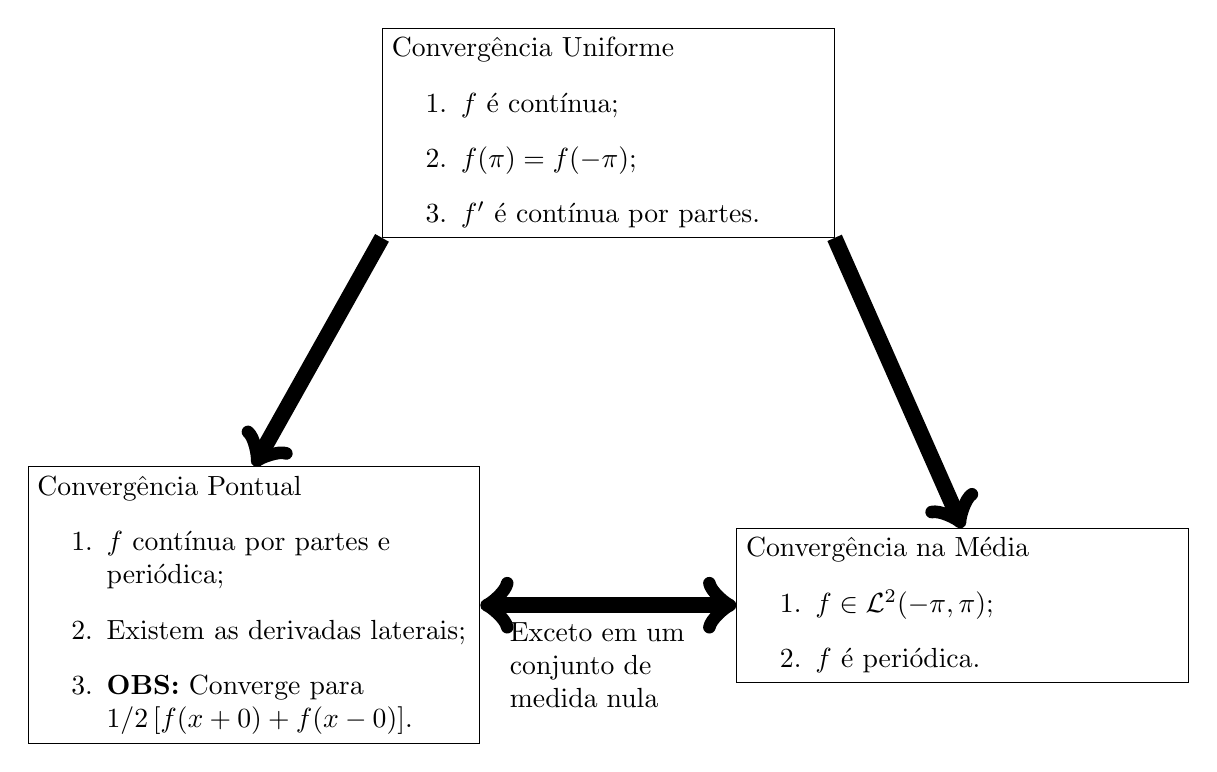
\begin{tikzpicture}
        \node[draw=black, text width=5.5cm] (U) at (0,0) {Converg\^{e}ncia Uniforme
        \begin{enumerate}
            \item $f$ \'{e} cont\'{i}nua;
            \item $f(\pi) = f(-\pi)$;
            \item $f'$ \'{e} cont\'{i}nua por partes.
        \end{enumerate}};
        \node[draw=black, text width=5.5cm] (P) at (-4.5,-6) {Converg\^{e}ncia Pontual
        \begin{enumerate}
            \item $f$ cont\'{i}nua por partes e peri\'{o}dica;
            \item Existem as derivadas laterais;
            \item \textbf{OBS:} Converge para $1/2 \left[ f(x + 0) + f(x - 0) \right]$.
        \end{enumerate}};
        \node[draw=black, text width=5.5cm] (M) at (4.5,-6) {Converg\^{e}ncia na M\'{e}dia
        \begin{enumerate}
            \item $f \in \mathcal{L}^2(-\pi, \pi)$;
            \item $f$ \'{e} peri\'{o}dica.
        \end{enumerate}};
        \draw[->, line width=.2cm] (U.south west) -- (P.north);
        \draw[->, line width=.2cm] (U.south east) -- (M.north);
        \draw[<->, line width=.2cm] (P.east) -- (M.west) node[midway, below, text width=2.5cm] {Exceto em um conjunto de medida nula};
    \end{tikzpicture}
\end{center}

\section{M\'{e}todo de Fej\'{e}r}
\begin{defi}
    Dadas as somas parciais $S_k(x) = \sum_{i = 0}^k \mu_i(x)$ para $k = 0, 1, \ldots, N - 1$, a soma de Ces\`{a}ro (ou m\'{e}dia C-1) \'{e} definida como a meia aritm\'{e}tica dessas somas parciais:
    \begin{align*}
        \sigma_N(x) &= \frac{1}{N} \sum_{k = 0}^{N - 1} S_k(x).
    \end{align*}
    Dizemos que uma s\'{e}rie \'{e} C-1 som\'{a}vel se existir o $\lim_{N \to \infty} \sigma_N(x)$.
\end{defi}
\begin{obs}
    Podemos definir a m\'{e}dia C-2, etc, como a m\'{e}dia aritm\'{e}tica das somas de Ces\`{a}ro, ou seja,
    \begin{align*}
        \sigma_N^{(2)}(x) &= \frac{1}{N} \sum_{k = 0}^{N - 1} \sigma_N(x),
    \end{align*}
    e dizer que a s\'{e}rie \'{e} C-2 som\'{a}vel se existir $\lim_{N \to \infty} \sigma_N^{(2)}(x)$.
\end{obs}
\begin{exem}
    Considere $S_k(x) = \sum_{i = 0}^{k - 1} (-1)^i$, ent\~{a}o
    \begin{align*}
        S_0 &= 1, \\
        S_1 &= 1 - 1 = 0, \\
        S_2 &= 1 - 1 + 1 = 1,
        \vdots
    \end{align*}
    e
    \begin{align*}
        S_0 &= 1, \\
        S_0 + S_1 &= 1, \\
        S_0 + S_1 + S_2 &= 2, \\
        \vdots
    \end{align*}
    Logo,
    \begin{align*}
        \sigma_0 &= \frac{1}{1} 1 = 1, & \sigma_1 &= \frac{1}{2} 1 = \frac{1}{2}, \\
        \sigma_2 &= \frac{1}{3} 2 = \frac{2}{3}, & \sigma_3 &= \frac{1}{4} 2 = \frac{1}{2}, \\
        \sigma_4 &= \frac{1}{5} 3 = \frac{3}{5}, & \sigma_5 &= \frac{1}{6} 3 = \frac{1}{2}, \\
        \vdots && \vdots \\
        \sigma_{2n} &= \frac{n + 1}{2n + 1}, & \sigma_{2n + 1} &= \frac{1}{2}.
    \end{align*}
    e como
    \begin{align*}
        & \lim_{n \to \infty} \sigma_{2n + 1} = 1/2, \\
        & \lim_{n \to \infty} \sigma_{2n} = 1/2,
    \end{align*}
    temos que a s\'{e}rie $\sum_{i = 0}^\infty (-1)^i$ \'{e} C-1 som\'{a}vel e o resultado \'{e} $1/2$.
\end{exem}
\begin{obs}
    Usar a soma de Ces\`{a}ro da s\'{e}rie de Fourier.
    \begin{align*}
        \sigma_1 &= \frac{a_0}{2}, \\
        \sigma_2 &= \frac{1}{2} \left[ \frac{a_0}{2} + \left[ \frac{a_0}{2} + \left( a_1 \cos\left( x \right) + b_1 \sin\left( x \right) \right) \right] \right], \\
        \begin{split}
            \sigma_3 &= \frac{1}{3} \left[ \frac{a_0}{2} + \left[ \frac{a_0}{2} + \sum_{k = 1}^1 \left( a_k \cos\left( k x \right) + b_k \sin\left( k x \right) \right) \right] \right. \\
            &\quad \left. {}+ \left[ \frac{a_0}{2} + \sum_{k = 1}^2 \left( a_k \cos\left( k x \right) + b_k \sin\left( k x \right) \right) \right] \right],
        \end{split} \\
        \vdots \\
        \begin{split}
            \sigma_N &= \frac{1}{N} \left[ \frac{a_0}{2} + \left[ \frac{a_0}{2} + \sum_{k = 1}^1 \left( a_k \cos\left( k x \right) + b_k \sin\left( k x \right) \right) \right] \right. \\
            &\quad {}+ \left[ \frac{a_0}{2} + \sum_{k = 1}^2 \left( a_k \cos\left( k x \right) + b_k \sin\left( k x \right) \right) \right] \\
            &\quad \vdots \\
            &\quad \left. {}+ \left[ \frac{a_0}{2} + \sum_{k = 1}^{N - 1} \left( a_k \cos\left( k x \right) + b_k \sin\left( k x \right) \right) \right]\right] \\
            &= \left( \frac{N}{N} \right) \left( \frac{a_0}{2} \right) + \left( \frac{N - 1}{N} \right) \left( a_1 \cos\left( x \right) + b_1 \sin\left( x \right) \right) \\
            &\quad {}+ \left( \frac{N - 2}{N} \left( a_2 \cos\left( 2 x \right) + b_2 \sin\left( 2 x \right) \right) \right) \\
            &\quad {}+ \cdots \\
            &\quad {}+ \left( \frac{N - \left( N - 1 \right)}{N} \right) \left( a_{N - 1} \cos\left( \left( N - 1 \right) x \right) + b_{N - 1} \sin\left( \left( N - 1 \right) x \right) \right) \\
        \end{split}
    \end{align*}
    Portanto,
    \begin{align*}
        \sigma_N(x) &= \frac{a_0}{2} + \sum_{k = 1}^{N - 1} \left( \alpha_k^N \cos\left( k x \right) + \beta_k^N \sin\left( k x \right) \right), \\
        \alpha_k^N &= \left( 1 - \frac{k}{N} \right) a_k, \\
        \beta_k^N &= \left( 1 - \frac{k}{N} \right) b_k.
    \end{align*}

    Por outro lado, sabemos que
    \begin{align*}
        S_N(x) &= \int_{-\pi}^\pi f(\xi) D_N(\xi - x) \id{\xi},
    \end{align*}
    onde $D_N$ denota o n\'{u}cleo de Dirichlet. Logo
    \begin{align*}
        \sigma_N(x) &= \frac{1}{N} \sum_{k = 0}^{N - 1} \int_{-\pi}^\pi f(\xi) D_k(\xi - x) \id{\xi}
    \end{align*}
    ou ainda
    \begin{align*}
        \sigma_N(x) &= \int_{-\pi}^\pi f(\xi) F_N(\xi - x) \id{\xi},
    \end{align*}
    onde
    \begin{align*}
        F_N(\mu) &= \frac{1}{N} \sum_{k = 0}^{N - 1} D_k(\mu).
    \end{align*}

    Lembrando que $D_k(\mu) = \left[ \sin\left( k + 1/2 \right) \mu \right] / \left[ 2 \pi \sin\left( \mu/2 \right) \right]$, temos
    \begin{align*}
        \sin^2\left( \mu/2 \right) F_N(\mu) &= \frac{1}{N} \sin^2\left( \mu/2 \right) \sum_{k = 0}^{N - 1} \frac{\sin\left( k + 1/2 \right) \mu}{2 \pi \sin\left( \mu/2 \right)} \\
        &= \frac{1}{2 \pi N} \sum_{k = 0}^{N - 1} \sin\left( \mu/2 \right) \sin\left( k + 1/2 \right) \mu \\
        &= \frac{1}{2 \pi N} \sum_{k = 0}^{N - 1} \frac{1}{2} \left[ \cos\left( k + 1/2 - 1/2 \right) \mu - \cos\left( k + 1/2 + 1/2 \right) \mu \right] \\
        &= \frac{1}{4 \pi N} \sum_{k = 0}^{N - 1} \left( \cos\left( k \mu \right) - \cos\left( \left( k + 1 \right) \mu \right) \right) \\
        &= \frac{1}{4 \pi N} \left( 1 - \cos\left( N \mu \right) \right) \\
        &= \frac{1}{2 \pi N} \left( \frac{1 - \cos\left( N \mu \right)}{2} \right) \\
        &= \frac{1}{2 \pi N} \sin^2\left( N \mu / 2 \right).
    \end{align*}
\end{obs}
\begin{defi}
    O n\'{u}cleo de Fej\'{e}r $F_N(\mu)$ \'{e} definido como
    \begin{align*}
        F_N(\mu) &= \frac{1}{N} \sum_{k = 0}^{N - 1} D_k(\mu) = \frac{\sin^2\left( N \mu / 2 \right)}{2 \pi N \sin^2\left( \mu/2 \right)}.
    \end{align*}
\end{defi}

Antes de prosseguir, \'{e} importante notermos que:
\begin{lem}
    Temos que
    \begin{align*}
        & \int_{-\pi}^\pi D_k(\mu) \id{\mu} = 1, \\
        & \int_{-\pi}^\pi F_k\left( \mu \right) \id{\mu} = 1.
    \end{align*}
\end{lem}
\begin{proof}
    Sabendo que
    \begin{align*}
        D_k(\mu) &= \frac{\sin\left( k + 1/2 \right) \mu}{2 \pi \sin\left( \mu/2 \right)} \\
        &= \left( 1 + 2 \sum_{j = 1}^{k - 1} \cos\left( j \mu \right) \right) \frac{1}{2 \pi}
    \end{align*}
    temos que
    \begin{align*}
        \int_{-\pi}^\pi D_k\left( \mu \right) \id{\mu} &= \frac{1}{2 \pi} \left[ \pi - \left( -\pi \right) + 2 \sum_{j = 1}^{k - 1} \left. \frac{\sin\left( j \mu \right)}{j} \right|_{-\pi}^\pi \right] = 1
    \end{align*}
    e
    \begin{align*}
        \int_{-\pi}^\pi F_k(\mu) \id{\mu} &= \frac{1}{k} \sum_{j = 0}^{k - 1} \int_{-\pi}^\pi D_j(\mu) \id{\mu} = \frac{1}{k} k = 1. \qedhere
    \end{align*}
\end{proof}
\begin{teo}[Fej\'{e}r] \label{teo:fejer}
    Seja $f(x)$ uma fun\c{c}\~{a}o cont\'{i}nua e peri\'{o}dica (de per\'{i}odo $2\pi$) e seja $\sigma_N(x)$ a soma de Ces\`{a}ro da s\'{e}rie de Fourier de $f(x)$, ou seja,
    \begin{align*}
        \sigma_N(x) &= \frac{a_0}{2} + \sum_{k = 1}^{N - 1} \left( \alpha_k^N \cos\left( k x \right) + \beta_k^N \sin\left( k x \right) \right),
    \end{align*}
    onde $\sigma_k^N = \left( 1 - k/N \right) a_k$ e $\beta_k^N = \left( 1 - k/N \right) b_k$. Ent\~{a}o a sequ\^{e}ncia de fun\c{c}\~{o}es $\sigma_n(x)$ converge para $f(x)$.
\end{teo}
\begin{proof}
    (mais f\'{a}cil que Fourier pois $F_N(\mu) \geq 0$)
    \begin{align*}
        \sigma_N(x) &= \int_{-\pi}^\pi f(\xi) F_N(\xi - x) \id{\xi} \\
        &= \int_{a - \pi}^{a + \pi} f(\xi) F_{N}(\xi - x) \id{\xi} \\
        &= \int_{x - \pi}^{x + \pi} f(\xi) F_N(\xi - x) \id{\xi} \\
        &= \int_{-\pi}^\pi f(x + \mu) F_N(\mu) \id{\mu} \\
        \sigma_N(x) - f(x) &= \int_{-\pi}^\pi f(x + \mu) F_N(\mu) \id{\mu} - f(x) \int_{-\pi}^\pi F_N(\mu) \id{\mu} \\
        &= \int_{-\pi}^\pi \left[ f(x + \mu) - f(x) \right] F_N(\mu) \id{\mu} \\
        &= \frac{1}{\pi N} \int_{-\pi}^\pi \left[ f(x + \mu) - f(x) \right] \frac{\sin^2\left( N \mu/2 \right)}{2 \sin^2\left( \mu/2 \right)} \id{\mu}
    \end{align*}
    Logo, como $f$ \'{e} cont\'{i}nua ent\~{a}o $\forall \epsilon > 0, \exists \delta > 0$ tal que $| f(x + \mu) - f(x)| < \epsilon$ para $| x + \mu - x| = | \mu | < \delta$.
    \begin{align*}
        | \sigma_N(x) - f(x)| &= \left| \int_{-\pi}^\pi \left( \ldots \right) \right| \\
        &= \left| \int_{-\pi}^{-\delta} \left( \ldots \right) + \int_{-\sigma}^\sigma \left( \ldots \right) + \int_\sigma^\pi \left( \ldots \right) \right| \\
        &\leq \underbrace{\left| \int_{-\pi}^{-\delta} \left( \ldots \right) \right|}_{|I_1|} + \underbrace{\left| \int_{-\sigma}^\sigma \left( \ldots \right) \right|}_{|I_2|} + \underbrace{\left| \int_\sigma^\pi \left( \ldots \right) \right|}_{|I_3|}
    \end{align*}
    Mas
    \begin{align*}
        |I_2| &\leq \int_{-\delta}^\delta \underbrace{| f(x + \mu) - f(x) |}_{< \epsilon} F_N(\mu) \id{\mu} \\
        &< \epsilon \int_{-\delta}^\delta \underbrace{F_N(\mu)}_{\geq 0} \id{\mu} \\
        &< \epsilon \underbrace{\int_{-\delta}^\delta F_N(\mu) \id{\mu}}_{=1} \\
        &< \epsilon, \\
        |I_1| &\leq  \frac{1}{\pi N} \int_{-\pi}^{-\delta} | f(x + \mu) - f(x) | \frac{\sin^2\left( N \mu/2 \right)}{2 \sin^2\left( \mu/2 \right)} \id{\mu} \\
        &\leq \frac{2 M}{\pi N} \int_{-\pi}^{-\delta} \frac{\sin^2\left( N \mu/2 \right)}{2 \sin^2\left( \mu/2 \right)} \id{\mu} \\
        \intertext{onde $M = \max |f(x)|$}
        &\leq \frac{2 M}{\pi N} \int_{-\pi}^{-\delta} \frac{1}{2 \sin^2\left( \mu/2 \right)} \id{\mu} \\
        &\leq \frac{2 M}{\pi N} \int_{-\pi}^{-\delta} \frac{1}{2 \sin^2\left( \delta/2 \right)} \id{\mu}\\
        &= \frac{M}{\pi N \sin^2\left( \delta/2 \right)} \underbrace{\int_{-\pi}^{-\delta} \id{\mu}}_{\pi - \delta < \pi} \\
        &\leq \frac{M \pi}{\pi N \sin^2\left( \delta/2 \right)} \\
        &\leq \frac{M}{N \sin^2\left( \delta/2 \right)}, \\
        \intertext{e analogamente}
        |I_3| &\leq \frac{M}{N \sin^2\left( \delta/2 \right)}.
    \end{align*}
    Portanto,
    \begin{align*}
        & |\sigma_N(x) - f(x)| \leq \epsilon + \frac{2 M}{N \sin^2\left( \delta/2 \right)}, \\
        & \lim_{N \to \infty} | \sigma_N(x) - f(x) | \leq \epsilon
    \end{align*}
    de onde conlu\'{i}mos que
    \begin{align*}
        \lim_{N \to \infty} \sigma_N(x) &= f(x) \qedhere
    \end{align*}
\end{proof}

\section{Diferencia\c{c}\~{a}o e Integra\c{c}\~{a}o}
\begin{teo}
    Seja $f(x)$ uma fun\c{c}\~{a}o cont\'{i}nua em $[-\pi,\pi]$ tal que $f(-\pi) = f(\pi)$ e seja $f'(x)$ cont\'{i}nua por partes e com derivadas laterais nesse intervalo. Ent\~{a}o a s\'{e}rie de Fourier de $f(x)$ \'{e} diferencia\'{a}vel e
    \begin{align*}
        f'(x) &= \sum_{n = 1}^\infty n \left( -a_n \sin\left( n x \right) + b_n \cos\left( n x \right) \right)
    \end{align*}
\end{teo}
\begin{proof}
    Como $f'(x)$ satisfaz as condi\c{c}\~{o}es do Teorema de Fourier (p\'{a}gina~\pageref{teo:fourier}), ela possui a s\'{e}rie de Fourier
    \begin{align*}
        f'(x) &= \frac{\alpha_0}{2} + \sum_{n = 1}^\infty \left( \alpha_n \cos\left( n x \right) + \beta_n \sin\left( n x \right) \right).
    \end{align*}
    Mas
    \begin{align*}
        \alpha_0 &= \frac{1}{\pi} \int_{-\pi}^\pi f'(x) \id{x} \\
        &= \frac{1}{\pi} \left[ f(\pi) - f(-\pi) \right] \\
        &= 0, \\
        \alpha_n &= \frac{1}{\pi} \left[ \underbrace{\left. f(x) \cos\left( n x \right) \right|_{-\pi}^\pi}_{=0} + n \int_{-\pi}^\pi f(x) \sin\left( n x \right) \id{x} \right] \\
        &= n b_n \\
        \beta_n &= \frac{1}{\pi} \left[ \underbrace{\left. f(x) \sin\left( n x \right) \right|_{-\pi}^\pi}_{=0} - n \int_{-\pi}^\pi f(x) \cos\left( n x \right) \id{x} \right] \\
        &= -n a_n
    \end{align*}
    de modo que
    \begin{align*}
        f'(x) &= \sum_{n = 1}^\infty \left( n b_n \cos\left( n x \right) - n a_n \sin\left( n x \right) \right). \qedhere
    \end{align*}
\end{proof}
\begin{obs}
    Note que o teorema fornece apenas uma condi\c{c}\~{a}o suficiente. Al\'{e}m disso, podemos ter s\'{e}rie de Fourier para $f(x)$ e n\~{a}o para $f'(x)$ (nesse caso o termo $n$ no numerador diminui a taxa de converg\^{e}ncia da s\'{e}rie).
\end{obs}
\begin{exem}
    A fun\c{c}\~{a}o $f(x) = x$ possui a s\'{e}rie de Fourier
    \begin{align*}
        x = 2 \sum_{n = 1}^\infty (-1)^{n + 1} \frac{\sin\left( n x \right)}{n}.
    \end{align*}
    Por\'{e}m $f(-\pi) = -\pi \neq \pi f(\pi)$, de modo que as condi\c{c}\~{o}es do teorema n\~{a}o s\~{a}o satisfeitas e nada podemos afirmar acerca da s\'{e}rie de Fourier de $f'(x)$ usando esse teorema. Note que nesse caso que a derivada da s\'{e}rie de Fourier n\~{a}o converge!
    \begin{align*}
        1 \neq 2 \sum_{n = 1}^\infty (-1)^{n + 1} \cos\left( n x \right).
    \end{align*}
\end{exem}
\begin{obs}
    Dentro das condi\c{c}\~{o}es do teorema anterior, uma vez que $\lim_{n \to \infty} \alpha_n = 0$ e $\lim_{n \to \infty} \beta_n = 0$ (crit\'{e}rio do termo geral), temos
    \begin{align*}
        \lim_{n \to \infty} n a_n &= 0, & \lim_{n \to \infty} n b_n &= 0.
    \end{align*}
    Note que a s\'{e}rie do exemplo anterior n\~{a}o satisfaz essas condi\c{c}\~{o}es.
\end{obs}
\begin{teo}
    Seja $f(x)$ uma fun\c{c}\~{a}o cont\'{i}nua por partes em $(-\pi,\pi)$. Ent\~{a}o, independentemente da s\'{e}rie de Fourier de $f(x)$ convergir ou n\~{a}o, vale a seguinte igualdade:
    \begin{align*}
        \int_{-\pi}^x f(\xi) \id{\xi} &= \frac{1}{2} a_0 \left( x + \pi \right) + \sum_{n = 1}^\infty \frac{1}{n} \left[ a_n \sin\left( n x \right) - b_n \left( \cos\left( n x \right) - \cos\left( n \pi \right) \right) \right],
    \end{align*}
    quando $x \in [-\pi,\pi]$.
\end{teo}
\begin{proof}
    Seja
    \begin{align*}
        F(x) &= \int_{-\pi}^x f(\xi) \id{\xi} - \frac{a_0}{2} x.
    \end{align*}
    Se $f(x)$ \'{e} cont\'{i}nua por partes ent\~{a}o $F(x)$ \'{e} cont\'{i}nua. Al\'{e}m disso $F'(x) = f(x) - a_0/2$, de modo que $F'(x)$ \'{e} cont\'{i}nua por partes. Podemos ainda notar que $F(-\pi) = -a_0 / 2 (-\pi) = \pi a_0 / 2$ e
    \begin{align*}
        F(\pi) &= \int_{-\pi}^\pi f(\xi) \id{\xi} - \frac{a_0}{2} \pi \\
        &= a_0 \pi - \frac{a_0}{2} \pi \\
        &= \frac{a_0 \pi}{2}
    \end{align*} 
    ou seja, $F(\pi) = F(-\pi)$. Temos com isso que $F(x)$ satisfaz as condi\c{c}\~{o}es do teorema de Fourier e possui portanto a s\'{e}rie de Fourier
    \begin{align*}
        F(x) &= \frac{A_0}{2} + \sum_{n = 1}^\infty \left( A_n \cos\left( n x \right) + B_n \sin\left( n x \right) \right), \\
        A_n &= \frac{1}{\pi} \int_{-\pi}^\pi F(x) \cos\left( n x \right) \id{x}, \\
        B_n &= \frac{1}{\pi} \int_{-\pi}^\pi F(x) \sin\left( n x \right) \id{x}.
    \end{align*}
    Para $n \neq 0$,
    \begin{align*}
        A_n &= \frac{1}{n} \int_{-\pi}^\pi \left[ \int_{-\pi}^x f(\xi) \id(\xi) - \frac{a_0}{2} x \right] \cos\left( n x \right) \id{x} \\
        &= \frac{1}{\pi} \underbrace{\left. F(x) \frac{\sin\left( n x \right)}{n} \right|_{-\pi}^\pi}_{=0} - \frac{1}{\pi} \int_{-\pi}^\pi \frac{\sin\left( n x \right)}{n} \left[ f(x) - \frac{a_0}{2} \right] \id{x} \\
        &= - \frac{1}{n \pi} \int_{-\pi}^\pi f(x) \sin\left( n x \right) \id{x} + \frac{a_0}{2 n \pi} \underbrace{\int_{-\pi}^\pi \sin\left( n x \right) \id{x}}_{=0} \\
        &= -\frac{1}{n} b_n, \\
        B_n &= \frac{1}{n} \int_{-\pi}^\pi \left[ \int_{-\pi}^x f(\xi) \id{\xi} - \frac{a_0 x}{2} \right] \sin\left( n x \right) \id{x} \\
        &= \underbrace{-\frac{1}{\pi} \left. F(x) \frac{\cos\left( n x \right)}{n} \right|_{-\pi}^\pi}_{=0} + \frac{1}{n \pi} \int_{-\pi}^\pi \cos\left( n x \right) \left[ f(x) - \frac{a_0}{2} \right] \id{x} \\
        &= \frac{1}{n \pi} \int_{-\pi}^\pi \cos\left( n x \right) f(x) \id{x} - \frac{a_0}{2 n \pi} \underbrace{\int_{-\pi}^\pi \cos\left( n x \right) \id{x}}_{=0} \\
        &= \frac{1}{n} a_n
    \end{align*}
    e portanto
    \begin{align*}
        F(x) &= \frac{A_0}{2} + \sum_{n = 1}^\infty \left( \frac{-b_n}{n} \cos\left( n x \right) + \frac{a_n}{n} \sin\left( n x \right) \right).
    \end{align*}
    Tomando $x = \pi$,
    \begin{align*}
        F(\pi) &= \frac{a_0 \pi}{2} = \frac{A_0}{2} \sum_{n = 1}^\infty \left( \frac{-b_n}{n} \cos\left( n \pi \right) + \frac{a_n}{n} \underbrace{\sin\left( n \pi \right)}_{=0} \right)
    \end{align*}
    e portanto
    \begin{align*}
        \frac{A_0}{2} &= \frac{a_0 \pi}{2} + \sum_{n = 1}^\infty \frac{b_n}{n} \cos\left( n \pi \right)
    \end{align*}
    de modo que
    \begin{align*}
        \int_{-\pi}^x f(\xi) \id{\xi} - \frac{a_0 x}{2} &= \frac{a_0 \pi}{2} + \sum_{n = 1}^\infty \frac{1}{n} \left[ a_n \sin\left( n x \right) - b_n \left( \cos\left( n x \right) - \cos\left( n \pi \right) \right) \right]. \qedhere
    \end{align*}
\end{proof}
\begin{obs}
    Note que no caso da integra\c{c}\~{a}o o termo $n$ no denominador aumenta a taxa de converg\^{e}ncia.
\end{obs}
\begin{exem}
    A s\'{e}rie de $f(x) = x$ \'{e}
    \begin{align*}
        x = 2 \sum_{n = 1}^\infty (-1)^{n + 1} \frac{\sin\left( n x \right)}{n}.
    \end{align*}
    Tomando $\int_0^x f(\xi) \id{\xi}$ temos
    \begin{align*}
        x^2 &= 4 \sum_{n = 1}^\infty \frac{(-1)^n}{n^2} \cos\left( n x \right) - 4 \sum_{n = 1}^\infty \frac{(-1)^n}{n^2}
    \end{align*}
    que \'{e} justamente a s\'{e}rie obtida na p\'{a}gina~\pageref{exem:fourier:x^2} uma vez que $\sum_{n = 1}^\infty (-1)^n / (n^2) = -\pi^2 / 12$.
\end{exem}

\section{Fen\^{o}meno de Gibbs}
Para ilustrar o fen\^{o}meno de Gibbs, vamos considerar uma onda quadrada peri\'{o}dica representada por
\begin{align*}
    f(x) &= \begin{cases}
        h/2, & 0 < x < \pi, \\
        -h/2, & -\pi < x < 0.
    \end{cases}
    1;3P
\end{align*}
e ilustrada na Figura
\begin{figure}[!htb]
    \centering
    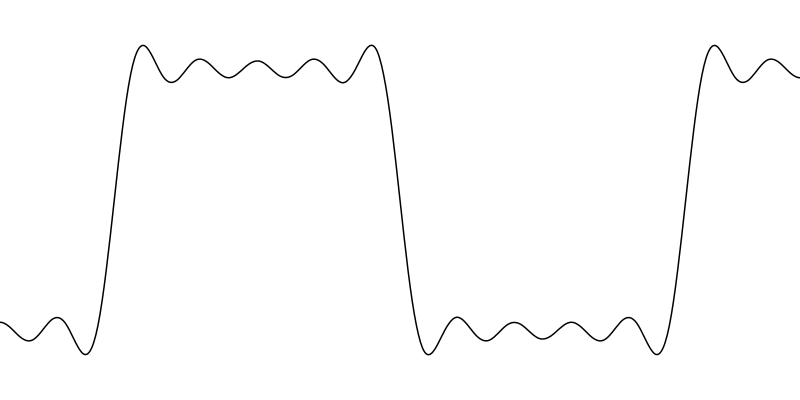
\includegraphics[width=.5\textwidth]{figuras/gibbs_phenomenon.png}
    \begin{flushright}
        Imagem em dom\'{i}nio p\'{u}blico de Johannes Rössel e dispon\'{i}vel em \url{http://en.wikipedia.org/wiki/File:Gibbs_phenomenon_10.svg}.
    \end{flushright}
    \caption{Ilustra\c{c}\~{a}o do Fen\^{o}meno de Gibbs para onda quadrada.}
    \label{fig:fenom_gibbs}
\end{figure}
% TODO Terminar de digitar a se\c{c}\~{a}o sobre o Fen\^{o}meno de Gibbs do arquivo M2S12-5.

\section{Teorema da Aproxima\c{c}\~{a}o de Weierstrass}
\begin{teo}
    Seja $f(x)$ cont\'{i}nua em $a \leq x \leq b$. Ent\~{a}o para todo $\epsilon > 0$ existe um polin\^{o}mio $P(x)$ tal que $|P(x) - f(x)| \leq \epsilon, \forall x \in [a,b]$.
\end{teo}
\begin{proof}
    Dado $f(x)$, $x \in [a,b]$, podemos definir $g(t)$ para $t \in [-\pi/2, \pi/2]$ atrav\'{e}s de
    \begin{align*}
        g(t) &= f\left[ \left( \frac{b - a}{\pi} t + \left( \frac{b - a}{2} \right) \right) \right].
    \end{align*}
    Podemos ainda definir uma extens\~{a}o de $g(t)$ para $x \in [-\pi, \pi]$, que denotaremos por $G(t)$, e de modo que $G(-\pi) = G(\pi)$. Podemos al\'{e}m disso considerar para os demais pontos a extens\~{a}o peri\'{o}dica de $G(t)$. Nessas condi\c{c}\~{o}es o Teorema de Fej\'{e}r (p\'{a}gina~\pageref{teo:fejer}) nos garante que a sequ\^{e}ncia $\sigma_N(t)$,
    \begin{align*}
        \sigma_N(t) &= \frac{a_0}{2} + \sum_{k = 1}^{N - 1} \left( \alpha_k^N \cos\left( k t \right) + \beta_k^N \sin\left( k t \right) \right),
    \end{align*}
    converge para $G(t)$, ou seja, $\forall \epsilon > 0$, existe $N_0 > 0$ tal que
    \begin{align*}
        | \sigma_N(t) - G(t) | < \epsilon/2
    \end{align*}
    para $N > N_0$. Por outro lado, pelo Teorema de Taylor, existem polin\^{o}mios $R_n^k(t)$ e $S_n^k(t)$ de grau $n$ tais que
    \begin{align*}
        | \cos\left( k t \right) - R_n^k(t) | &< \epsilon', & | \sin\left( k t \right) - S_n^k(t) | &< \epsilon'',
    \end{align*}
    para $n > N_1$. Portanto, existe um polin\^{o}mio $Q_N(t)$, que \'{e} uma combina\c{c}\~{a}o dos polin\^{o}mios $R_n^k(t)$ e $S_n^k(t)$, tal que
    \begin{align*}
        | \sigma_N(t) - Q_N(t) | < \epsilon/2.
    \end{align*}
    Com isso,
    \begin{align*}
        | G(t) - Q_N(t) | &= | G(t) - \sigma_N(t) + \sigma_N(t) - Q_N(t) | \\
        &\leq \underbrace{| G(t) - \sigma_N(t) |}_{< \epsilon/2} + \underbrace{| \sigma_N(t) - Q_N(t) |}_{< \epsilon/2}
    \end{align*}
    e portanto $| G(t) - Q_N(t) | < \epsilon$ para $t \in [-\pi, \pi]$ e $| g(t) - Q_N(t) | < \epsilon$ para $t \in [-\pi/2, \pi/2]$ ou, definindo $P_N(x) = Q_N\left[ \left( \pi / \left( b - a \right) \right) x - \left( \pi / 2 \right) \left( \left( b + a \right) / \left( b - a \right) \right) \right]$,
    \begin{align*}
        | f(x) - P_N(x) | < \epsilon
    \end{align*}
    para $x \in [a, b]$.
\end{proof}

\chapter{Série de Fourier Generalizadas}
\section{O Problema de Sturm-Liouville (PSL)}
Vamos recordar alguns fatos básicos sobre o PSL. Seja
\begin{align*}
    L[y] &= \frac{\id{}}{\id{x}}\left[ p(x) \frac{\id{y}}{\id{x}} \right] - q(x) y.
\end{align*}
O PSL consiste na equação diferencial
\begin{align*}
    L[y] + \lambda p(x) y &= 0, & a \leq x \leq b
\end{align*}
com condições apropriadas conforme o problema seja regular ou singular. Uma solução $y$ não-trivial é dita uma auto-função e a constante $\lambda$ correspondente um auto-valor.

O PSL regular corresponde ao caso em que $p(x) > 0$, $\rho(x) > 0$, $p, p', q, \rho$ são contínuas em $x \in [a,b]$. Nesse caso as condições adequadas são:
\begin{enumerate}
    \item para condições de contorno homogêneas:
        \begin{align*}
            \begin{cases}
                \alpha_1 y(a) + \beta_1 y'(a) = 0, \\
                \alpha_2 y(b) + \beta_2 y'(b) = 0.
            \end{cases}
        \end{align*}
    \item para condições periódicas:
        \begin{align*}
            \begin{cases}
                y(a) = y'(b), \\
                y'(a) = y'(b).
            \end{cases}
        \end{align*}
    \item $y$ e $y'$ são limitadas (para $x \to a$ ou $x \to \pm \infty$ conforme o caso).
\end{enumerate}

E o PSL singular corresponde as
\begin{enumerate}
    \item $p(a) = 0$ ou $p(a) = 0$ e/ou $p(b) = 0$ ou $p(b) = 0$.
    \item $-\infty < x < \infty$, $0 \leq x \leq \infty$ e $-\infty < x \leq 0$.
\end{enumerate}

\begin{teo}
    As autofunções correspondentes a diferentes autovalores de um PSL regular com condição de contorno homoêneas ou periódicas são ortogonais com peso $\rho(x)$ em $[a,b]$, ou seja,
    \begin{align*}
        \int_a^b \rho(x) u(x) v(x) \id{x} = 0.
    \end{align*}
    O mesmo vale para as autofunções de quadrado integrável de um PSL singular com a condição que estas autofunções e suas derivadas primeiras sejam limitadas nos extremos.
\end{teo}
\begin{proof}
    % TODO Escrever prova.
    Ver curso de MS410.
\end{proof}
\begin{exem}
    Considere o PSL dado por
    \begin{align*}
        \begin{cases}
            y'' + \lambda y = 0, & -\pi < x < \pi, \\
            y(-\pi) = y(\pi), \\
            y(-\pi) = y'(\pi).
        \end{cases}
    \end{align*}

    Esse PSL tem autovalores $\lambda = n^2$, para $n = 0, 1, 2, \ldots$ e auto-funções $\left\{ 1, \cos\left( n x \right), \sin\left( n x \right) \right\}$. Note que temos duas autofunções para o mesmo autovalor para $n = 1, 2, \ldots$. Logo, os autovalores não são simples no caso periódico.

    Denotando
    \begin{align*}
        \phi_1(x) &= 1, & \phi_{2n}(x) &= \sin\left( n x \right), & \phi_{2n + 1}(x) &= \cos\left( n x \right)
    \end{align*}
    para $n = 1, 2, \ldots$ temos que o auto-valor correspondente a $\phi_k(x)$ é
    \begin{align*}
        \lambda_k &= \left( \left[ \frac{k}{2} \right] - 1 \right)^2
    \end{align*}
    onde $\left[ a \right]$ denota a parte inteira de $a$.

    A relação de ortogonalidade é
    \begin{align*}
        \int_{-\pi}^\pi \phi_n(x) \phi_m(x) \id{x} &= 0,
    \end{align*}
    para $n \neq m$, ou seja, as autofunções são ortogonais com peso $\rho(x) = 1$.
\end{exem}
\begin{exem}
    Considere o PSL dado por
    \begin{align*}
        \begin{cases}
            \left[ \left( 1 - x^2 \right) y' \right]' + \lambda y = 0, & -1 < x < 1 \\
            \lim_{x \to \pm 1} | y(x) | < \infty, \\
            \lim_{x \to \pm 1} | y'(x) | < \infty.
        \end{cases}
    \end{align*}

    Esse é um PSL singular cujos autovalores são $\lambda = n \left( n + 1 \right)$ para $n = 0, 1, 2, \ldots$ e as correspondentes autofunções são os polinômios de Legendre $P_n(x)$ definidos por
    \begin{align*}
        P_n(x) &= \frac{1}{2^n n!} \frac{\id{}^n}{\id{x^n}}\left( x^2 - 1 \right)^n
    \end{align*}
    para $n = 1, 2, \ldots$ e $P_0(x) = 1$. Logo,
    \begin{align*}
        P_1(x) &= x, \\
        P_2(x) &= \left( 1/2 \right) \left( 3 x^2 - 1 \right), \\
        P_3(x) &= \left( 1/2 \right) \left( 5 x^3 - 3 x \right), \ldots
    \end{align*}
\end{exem}

\section{Expansão ortogonais}
Sejam $\left\{ \phi_n(x) \right\}$ para $n = 1, 2, \ldots$ funções de quadrado integrável com peso $\rho(x)$ em $[a,b]$,
\begin{align*}
    \int_a^b \rho(x) \left[ \phi_n(x) \right]^2 \id{x} < \infty
\end{align*}
e ortogonais (com peso $\rho(x)$) para $n \neq m$,
\begin{align*}
    \int_a^b \rho(x) \phi_n(x) \phi_m(x) \id{x} = 0
\end{align*}
para $n \neq m$.

Vamos denotar por $\langle \cdot, \cdot \rangle$ o produto escalar em $L_p^2(a, b)$:
\begin{align*}
    \langle f,g \rangle &= \int_a^b \rho(x) f(x) g(x) \id{x}.
\end{align*}

Agora vamos supor que uma função $f(x)$ pode ser escrita como o limite de uma série uniformimente convergente de múltiplos de $\phi_n(x)$, ou seja,
\begin{align*}
    f(x) &= \sum_{k = 1}^\infty c_n \phi_n(x).
\end{align*}
Com isso temos que
\begin{align*}
    \langle f,\phi_m \rangle &= \int_a^b \rho(x) f(x) \phi_m(x) \id{x} \\
    &= \int_a^b \left( \sum_{n = 1}^\infty c_n \phi_n(x) \right) \phi_m(x) \rho(x) \id{x} \\
    &= \sum_{n = 1}^\infty c_n \int_a^b \phi_n(x) \phi_m(x) \rho(x) \id{x} \\
    &= \sum_{n = 1}^\infty c_n \delta_{nm} \int_a^b \left[ \phi_m(x) \right]^2 \rho(x) \id{x} \\
    &= c_n \int_a^b \left[ \phi_m(x) \right]^2 \rho(x) \id{x} \\
    &= c_m \langle \phi_m, \phi_m \rangle \\
    &= c_m \| \phi_m \|^2,
\end{align*}
ou seja,
\begin{align*}
    c_n &= \frac{\langle f, \phi_n \rangle}{\| \phi_n \|^2}.
\end{align*}

\begin{exem}
    Para a série de Fourier temos
    \begin{align*}
        \| \phi_1(x) \|^2 &= 2 \pi, & \| \phi_k \|^2 &= \pi
    \end{align*}
    para $k = 2, 3, \ldots$, e portanto
    \begin{align*}
        c_1 &= \frac{\langle f, \phi_1 \rangle}{2\pi} \\
        &= \frac{1}{2\pi} \int_{-\pi}^\pi f(x) \id{x} \\
        &= \frac{a_0}{2}, \\
        c_{2n} &= \frac{\langle f, \phi_{2n} \rangle}{\pi} \\
        &= \frac{1}{\pi} \int_{-\pi}^\pi f(x) \sin\left( n x \right) \id{x} \\
        &= b_n, \\
        c_{2n + 1} &= \frac{\langle f, \phi_{2n + 1} \rangle}{\pi} \\
        &= \frac{1}{\pi} \int_{-\pi}^\pi f(x) \cos\left( n x \right) \id{x} \\
        &= a_n.
    \end{align*}
\end{exem}

Diremos que $c_n$ é o coeficiente de Fourier generalizado da série de Fourier generalizada $f(x) = \sum_{n = 1}^\infty c_n \phi_n(x)$.

Dada uma soma
\begin{align*}
    s_N(x) &= \sum_{n = 1}^N \gamma_n \phi_n(x),
\end{align*}
o desvio total quadrático $\Delta_N$
\begin{align*}
    \Delta_N &= \| s_N - f \|^2 \\
    &= \int_a^b \rho(x) \left[ s_N(x) - f(x) \right]^2 \id{x}
\end{align*}
é minimizado quando $\gamma_n = c_n$, ou seja, $s_N = S_N$, que é a $N$-ésima soma parcial da série de Fourier generalizada. De fato:
\begin{align*}
    \Delta_N &= \langle s_N - f, s_N - f \rangle \\
    &= \langle s_N, s_N \rangle - 2 \langle s_N, f \rangle - \langle f, f \rangle, \\
    \langle s_N, s_N \rangle &= \sum_{n = 1}^`N \sum_{m = 1}^N \gamma_n \gamma_m \langle \phi_n, \phi_m \rangle \\
    &= \sum_{n = 1}^N \gamma_n^2 \| \phi_n \|^2, \\
    \langle s_N, f \rangle &= \sum_{n = 1}^N \gamma_n \langle \phi_n, f \rangle.
\end{align*}
Portanto,
\begin{align*}
    \frac{\partial \Delta_N}{\partial \gamma_k} &= 2 \gamma_k \| \phi_k \|^2 - 2 \langle \phi_k, f \rangle = 0
\end{align*}
que implica em
\begin{align*}
    \gamma_k = \frac{\langle \phi_k, f \rangle}{\| \phi_k \|^2} &= c_k.
\end{align*}

Como $\Delta_N \geq 0$, para $\Delta_N^{\min{}}$ temos
\begin{align*}
    0 \leq \Delta_N^{\min{}} \\
    &= \sum_{n = 1}^N c_n^2 \| \phi_n \|^2 - 2 \sum_{n = 1}^N c_n \langle \phi_n, f \rangle + \| f \|^2 \\
    &= \sum_{n = 1}^N \frac{\langle \phi_n, f \rangle^2}{\| \phi_n \|^2} \| \phi_n \|^2 - 2 \sum_{n = 1}^\infty \frac{\langle \phi_n, f \rangle}{\| \phi_n \|^2} + \| f \|^2,
\end{align*}
ou seja,
\begin{align*}
    \sum_{n = 1}^N \frac{\langle \phi_n, f \rangle^2}{\| \phi_n \|^2} \leq \| f \|^2
\end{align*}
e com os argumentos conhecidos para a série de Fourier segue a desigualdade de Bessel generalizada
\begin{align*}
    \sum_{n = 1}^\infty \frac{\langle \phi_n, f \rangle^2}{\| \phi_n \|^2} \leq \| f \|^2.
\end{align*}

Dizemos que $S_N(x)$ converge na média para $f(x)$ se
\begin{align*}
    \lim_{N \to \infty} \| S_N - f \|^2 &= \lim_{N \to \infty} \left\| \sum_{n = 1}^N c_n \phi_n - f \right\|^2 = 0
\end{align*}
e nesse caso dizemos que $\left\{ \phi_n(x) \right\}$ é completo. Uma condição necessária e suficiente para isso é valer a identidade de Parseval generalizada,
\begin{align*}
    \sum_{n = 1}^\infty \frac{\langle \phi_n, f \rangle^2}{\| \phi_n \|^2} &= \| f \|^2,
\end{align*}
ou ainda
\begin{align*}
    \sum_{n = 1}^\infty c_n^2 \| \phi_n \|^2 &= \| f \|^2.
\end{align*}

\section{Polinômios ortogonais}
% TODO Terminar de incluir arquivo M2S12-6.pdf. Interrompido na página 76.
% TODO Incluir arquivo M2S12-7.pdf
